\documentclass[a4paper,12pt]{article}
\usepackage[russian]{babel}
\usepackage[T2A]{fontenc}
\usepackage[utf8]{inputenc}
\usepackage{geometry}
\usepackage{amsmath}
\usepackage{graphicx}
\usepackage{cancel}
\usepackage{float} 
\usepackage{xcolor}
\usepackage{array}
\usepackage{caption}
\usepackage{booktabs}
\usepackage{amssymb}
\usepackage{subcaption}
\usepackage{pgfplots}
\pgfplotsset{compat=1.18}
\usetikzlibrary{arrows.meta, matrix}
\usepackage{capt-of}
\usepackage{multirow}
\usepackage[siunitx]{circuitikz}
\usepackage[bottom]{footmisc}
\usepackage{tcolorbox}
\usepackage{nicematrix}
\usepackage{tikz}
\usetikzlibrary{positioning, arrows.meta}

% --- hyperref ОДИН РАЗ ---
\usepackage{hyperref}
\hypersetup{linktoc=page}
\hypersetup{
	colorlinks=true,
	linkcolor=red,
	citecolor=red,
	urlcolor=red,
	filecolor=red,
}

% --- Содержание ---
\usepackage{tocloft}
\usepackage{etoolbox}
\usepackage{hyperref}
\hypersetup{
	colorlinks=true,
	linkcolor=red,
	citecolor=red,
	urlcolor=red,
}

% Патчим \tableofcontents: текст строк — без ссылок и чёрный
% Это делается через замену \contentsline внутри TOC
\preto\tableofcontents{%
	\begingroup
	% Переопределяем contentsline так, чтобы текст был чёрным без ссылки,
	% а номер страницы — красной ссылкой
	\renewcommand{\contentsline}[4]{%
		\ifnum\pdfstrcmp{##1}{section}=0
		\vskip 4pt{\normalfont\color{black}##2}\nobreak\hfill
		{\normalfont\color{red}\hyperlink{##4}{##3}}\par
		\else\ifnum\pdfstrcmp{##1}{subsection}=0
		\vskip 2pt\hspace{1.5em}{\normalfont\color{black}##2}\nobreak\hfill
		{\normalfont\color{red}\hyperlink{##4}{##3}}\par
		\else
		\vskip 1pt\hspace{3em}{\normalfont\color{black}##2}\nobreak\hfill
		{\normalfont\color{red}\hyperlink{##4}{##3}}\par
		\fi\fi
	}%
}
\appto\tableofcontents{\endgroup}

% tocloft — только для отступов, без переопределения шрифтов
\usepackage{tocloft}

% --- Листинги ---
\usepackage{listings}

\definecolor{codebg}{RGB}{250,250,252}
\definecolor{linenumcolor}{RGB}{150,150,170}
\definecolor{mathblue}{RGB}{30,100,200}
\definecolor{mathorange}{RGB}{200,100,20}
\definecolor{matlabblue}{RGB}{0,0,200}
\definecolor{matlabgreen}{RGB}{30,130,30}
\definecolor{matlaborange}{RGB}{200,80,0}

\lstdefinelanguage{Mathematica}{
	keywords={Plot, Eigenvalues, MatrixExp, RiccatiSolve, IdentityMatrix,
		Inverse, Transpose, Simplify, Eigensystem, StateSpaceModel,
		ControllabilityMatrix, MatrixRank, Export, FileNameJoin,
		NotebookDirectory, ConstantArray, ZeroMatrix, NDSolve,
		Evaluate, LineLegend, Placed, Directive, Opacity, Filling,
		FillingStyle, PlotStyle, PlotLegends, PlotRange, Frame,
		Axes, FrameLabel, GridLines, GridLinesStyle, AspectRatio,
		Style, FontFamily, FontSize, Thick, Dashed, Dotted,
		DotDashed, RGBColor, GrayLevel, LegendLayout, LabelStyle,
		Subscript, Table, Do, Module, Block, If, True, False, Automatic},
	sensitive=true,
	morecomment=[s]{(*}{*)},
	morestring=[b]",
}

\lstdefinestyle{mma}{
	language=Mathematica,
	basicstyle=\ttfamily\small,
	keywordstyle=\color{mathblue}\bfseries,
	commentstyle=\color{linenumcolor}\itshape,
	stringstyle=\color{mathorange},
	numberstyle=\tiny\color{linenumcolor},
	numbers=left,
	numbersep=10pt,
	backgroundcolor=\color{codebg},
	frame=single,
	frameround=tttt,
	framesep=4pt,
	rulecolor=\color{mathblue!40},
	breaklines=true,
	tabsize=4,
	showstringspaces=false,
	captionpos=b,
	xleftmargin=15pt,
	xrightmargin=5pt,
}

\lstdefinestyle{matlab}{
	language=Matlab,
	basicstyle=\ttfamily\small,
	keywordstyle=\color{matlabblue}\bfseries,
	commentstyle=\color{matlabgreen}\itshape,
	stringstyle=\color{matlaborange},
	numberstyle=\tiny\color{linenumcolor},
	numbers=left,
	numbersep=10pt,
	backgroundcolor=\color{codebg},
	frame=single,
	frameround=tttt,
	framesep=4pt,
	rulecolor=\color{matlabblue!30},
	breaklines=true,
	tabsize=4,
	showstringspaces=false,
	captionpos=b,
	xleftmargin=15pt,
	xrightmargin=5pt,
	escapeinside={\%*}{*)},
	morekeywords={cvx_begin,cvx_end,sdp,variable,minimize,maximize},
}

\lstset{style=mma}

\renewcommand{\lstlistingname}{Листинг}
\DeclareCaptionFormat{redlisting}{#1\textcolor{red}{#2}#3}
\captionsetup[lstlisting]{format=redlisting}

\geometry{left=1.5cm, right=2cm, bottom=2cm, top=2cm}
\captionsetup[figure]{name=Рисунок}
\captionsetup[table]{name=Таблица}
\captionsetup{labelsep=endash}


\begin{document}
	
	\begin{titlepage}
		\centering
		
		\vspace*{0.5cm}
		{\small
			Министерство науки и высшего образования Российской Федерации\\[2pt]
			Федеральное государственное автономное образовательное учреждение\\
			высшего образования\\[2pt]
			\textbf{«Национальный исследовательский университет ИТМО»}\\
		}
		
		\vspace{0.8cm}
		\hrule height 0.8pt
		\vspace{0.3cm}
		
		{\large Факультет систем управления и робототехники}
		
		\vspace{0.3cm}
		\hrule height 0.4pt
		\vspace{2.5cm}
		
		{\Huge\bfseries ОТЧЁТ}\\[0.4cm]
		{\LARGE\bfseries о лабораторной работе}\\[0.8cm]
		
		\begin{tcolorbox}[
			colback=gray!4,
			colframe=gray!10,
			boxrule=0.8pt,
			arc=4pt,
			left=12pt, right=12pt, top=8pt, bottom=8pt
			]
			\centering
			{\large По дисциплине:\\[4pt]}
			{\large\bfseries «Теория автоматического управления»}\\[10pt]
			{\large Тема:\\[4pt]}
			{\large\bfseries «Регуляторы с заданной степенью устойчивости»} \\[10pt]
			{\large Поток: 1.1.3 \( \) Вариант: 25}
		\end{tcolorbox}
		
		\vspace{3cm}
		
		\begin{minipage}{0.45\textwidth}
			\raggedright
			{\large\bfseries Студент:}\\[4pt]
			Охрименко Е.\,Д.\\
		\end{minipage}
		\hfill
		\begin{minipage}{0.45\textwidth}
			\raggedleft
			{\large\bfseries Преподаватель:}\\[4pt]
			Пашенко А.\,В.\\
		\end{minipage}
		
		\vfill
		\vspace{0.4cm}
		{\large Санкт-Петербург, 2026}
	\end{titlepage}
	
	\newpage
	\tableofcontents
	
	\newpage \section{Синтез регулятора с заданной степенью устойчивости}\label{sec:1}
	
	В соответствии с вариантом рассмотрю систему:
	\[
	\dot x = \begin{bmatrix}
		8 & 1 & 11 \\
		4 & 0 & 4 \\
		-4 & -3 & -7 \\
	\end{bmatrix} x + \begin{bmatrix}
	-1 \\ -3 \\ 3 \\
	\end{bmatrix} u
	\]
	
	Требуется:
	\begin{enumerate}
		\item Найти собственные числа матрицы $A$ и определить управляемость системы.
		
		\item Определить достижимую степень устойчивости при регуляторе $u = Kx$.
		
		\item Построить схему моделирования замкнутой системы.
		
		\item Выбрать несколько значений желаемой степени устойчивости $\alpha$.
		
		\item Для каждого $\alpha$ синтезировать регуляторы $K_1$, $K_2$ по неравенству Ляпунова, определить собственные числа $(A+BK)$ и выполнить моделирование.
		
		\item Для каждого $\alpha$ синтезировать регуляторы $K_3$, $K_4$ по уравнению Риккати, определить собственные числа $(A+BK)$ и выполнить моделирование.
		
		\item Сравнить результаты и сделать выводы.
	\end{enumerate}
	
	\hrule \newpage
	
	\subsection{Анализ матрицы системы}
	
	Найду собственные числа матрицы \(A\):
	\[
	\operatorname{det}(\lambda I - A) = \operatorname{det}\begin{bmatrix}
		\lambda-8 & -1 & -11\\
		-4 & \lambda & -4\\
		4 & 3 & \lambda+7
	\end{bmatrix} = \lambda^3-\lambda^2+4\lambda+24 = 0
	\]
	
	\[
	\sigma(A) = \{-3,\; 2 \pm 2\mathrm{j}\}
	\]
	
	Определю управляемость системы. Матрица управляемости системы (листинг~\ref{lst:U1}):
	\[
	U = \begin{bmatrix}
		 -1 & 22 & 96 \\
		-3 & 8 & 56 \\
		3 & -8 & -56 \\
	\end{bmatrix} \qquad \Longrightarrow \qquad
	\operatorname{rank}(U) = 2
	\]
	
	Система не полностью управляема, так как ранг матрицы управляемости меньше ранга матрицы системы.
	
	Для определения управляемости собственных чисел переведу систему в жорданов базис (листинг~\ref{lst:jordan1}). Получаю:
	\[
	\dot{\hat x} = \begin{bmatrix}
		-3 & 0 & 0 \\
		0 & 2 & 2 \\
		0 & -2 & 2 \\
	\end{bmatrix} \hat x + \begin{bmatrix}
		0 \\ 3/2 \\ -7/2 \\
	\end{bmatrix} u
	\]
	
	Собственное число \(\lambda_1 = -3\) не управляемо, так как ему соответствует нулевой элемент матрицы \(\hat B\). Неуправляемое собственное число отрицательно, поэтому система стабилизируема.	
	
	\subsection{Достижимая степень устойчивости}
	
	Регулятор $u = Kx$ может перемещать только управляемые собственные 
	числа матрицы $A$. Собственное число $\lambda_1 = -3$ неуправляемо 
	и остаётся фиксированным при любом выборе $K$.
	
	Степень устойчивости определяется как:
	\[
	\alpha = \min_i \, |\operatorname{Re}(\lambda_i)|
	\]
	то есть равна расстоянию от ближайшего собственного числа до мнимой оси.
	
	Поскольку $\lambda_1 = -3$ неуправляемо и зафиксировано, 
	максимально достижимая степень устойчивости:
	\[
	\alpha_{\max} = 3
	\]
	
	В качестве желаемых степеней устойчивости выберу два значения: $\alpha_1 = 0.5$ и $\alpha_2 = 3$.
	
	\subsection{Структурная схема системы}
	
	Замкну систему регулятором $u = Kx$, подставив в уравнение системы:
	\[
	\dot{x} = Ax + Bu = Ax + BKx = (A + BK)x
	\]
	
\begin{figure}[H]
	\centering
	\begin{tikzpicture}[
		block/.style={draw, rectangle, minimum width=2cm, minimum height=0.8cm,
			align=center, fill=blue!8, rounded corners=2pt, thick},
		intblock/.style={draw, rectangle, minimum width=0.8cm, minimum height=0.8cm,
			align=center, fill=orange!15, rounded corners=2pt, thick},
		arrow/.style={-{Stealth[length=2mm]}, thick},
		]
		
		\node[block]   (ABK) at (0, 0)   {$A + BK$};
		\node[intblock] (int) at (3, 0)  {$\dfrac{1}{s}$};
		\node[right=1.5cm of int] (xout) {$x(t)$};
		
		\draw[arrow] (ABK) -- node[above]{\small$\dot{x}$} (int);
		\draw[arrow] (int) -- node[above]{\small$x$} (xout);
		
		% Обратная связь
		\coordinate (branch) at ($(int.east)+(0.7,0)$);
		\draw[thick] (int.east) -- (branch);
		\draw[arrow] (branch) -- ++(0,-1.2) -| node[below, near start]{\small$x$} (ABK.south);
		
	\end{tikzpicture}
	\caption{Схема моделирования замкнутой системы}
\end{figure}


	\subsection{Синтез регуляторов матричным неравенством типа Ляпунова}
	
	Чтобы синтезировать регулятор, решу матричное неравенство типа Ляпунова для усеченной системы в жордановом базисе. Затем перейду в исходный базис и расширю систему. Управляемая часть системы в жордане:
	\[
	\begin{aligned}
		\hat A &= \begin{bNiceMatrix}[create-medium-nodes,left-margin=4pt,right-margin=4pt]
			-3 & 0 & 0 \\
			0 & 2 & 2 \\
			0 & -2 & 2 \\
			\CodeAfter
			\tikz \draw[red!80!black,line width=0.7pt,opacity=0.4]
			([xshift=-2pt]1-1-medium.west) -- ([xshift=2pt]1-3-medium.east);
			\tikz \draw[red!80!black,line width=0.7pt,opacity=0.4]
			([yshift=2pt]1-1-medium.north) -- ([yshift=-2pt]3-1-medium.south);
		\end{bNiceMatrix} \\[8pt]
		\hat B &= \begin{bNiceMatrix}[create-medium-nodes,left-margin=4pt,right-margin=4pt]
			0 \\ 3/2 \\ -7/2 \\
			\CodeAfter
			\tikz \draw[red!80!black,line width=0.7pt,opacity=0.4]
			([yshift=2pt]1-1-medium.north) -- ([yshift=-2pt]1-1-medium.south);
		\end{bNiceMatrix}
	\end{aligned}
	\qquad \Longrightarrow \qquad
	\begin{aligned}
		\hat A_c &= \begin{bmatrix} 2 & 2 \\ -2 & 2 \end{bmatrix} \\[28pt]
		\hat B_c &= \begin{bmatrix} 3/2 \\ -7/2 \end{bmatrix}
	\end{aligned}
	\]
	
	\subsubsection{Степень устойчивости $\alpha_1=0.5$}
	
	Синтезирую регулятор без ограничений на управление. Решу матричное неравенство Ляпунова для усечённой системы:
	\[
	\begin{cases}
		P \hat A_c^T + \hat A_c P + 2\alpha_1 P + Y^T \hat B_c^T + \hat B_c Y \preceq 0 \\
		P \succ 0 \\
		\hat K_\text{1,c} = YP^{-1} \\
	\end{cases}
	\]
	
	Решаю LMI в \texttt{cvx} (листинг~\ref{lst:cvx1}). Получаю:
	\[
	\begin{array}{rcl}
		P &=& \begin{bmatrix} 
			4.04 & -3.61 \\
			-3.61 & 4.67
		\end{bmatrix} \\[16pt]
		Y &=& \begin{bmatrix} -2.64 & 6.17 \end{bmatrix}
	\end{array}
	\qquad \Longrightarrow \qquad
	\hat{K}_{1,c} = YP^{-1} = \begin{bmatrix} 1.69 & 2.63 \end{bmatrix}
	\]

	Дополняю матрицу \(\hat{K}_{1,c}\) нулём для неуправляемого собственного числа и перехожу в исходный базис (листинг~\ref{lst:K1}):
	\[
		\hat{K_1} = \begin{bmatrix} 0 & 1.69 & 2.63 \end{bmatrix} 
		\qquad \Longrightarrow \qquad 
		K_1 = \hat{K_1} \cdot P_j^{-1} = \begin{bmatrix} -2.63 & 0.47 & -2.63 \end{bmatrix} 
	\]
	
	Проверяю спектр замкнутой системы (листинг~\ref{lst:lEig1}):
	\[
	\sigma(A + BK_1) = \{-1.3 \pm 3.55\mathrm{j},\; -3\}
	\]
	
	Построю графики вектора состояния \(x(t)\) при начальных условиях \(x(0) = \begin{bmatrix} 1 & 1 & 1 \\ \end{bmatrix}^T\) для степени устойчивости \(\alpha_1 = 0.5\) без ограничений на управление.
	
	\begin{figure}[H]
		\centering
		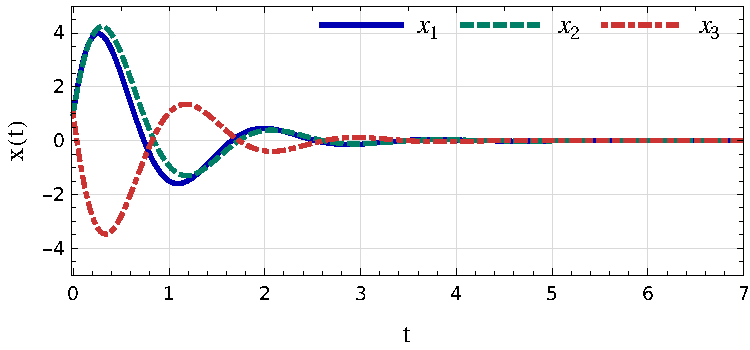
\includegraphics[width=0.7\textwidth]{../images/task1/Xa1K1L.pdf}
		\caption{Вектор состояния $x(t)$ при отсутствии ограничений на управление}
	\end{figure}
	
	Синтезирую регулятор совместно с решением задачи минимизации управления (листинг~\ref{lst:cvxmin1}). Получившаяся усеченная матрица регулятора в жордановом базисе:
	\[
	\hat{K}_{2,c} = YP^{-1} = \begin{bmatrix} 0.99 & 1.85 \end{bmatrix}
	\]
	
	Перейду в расширенный исходный базис (листинг~\ref{lst:K1}, аналогично):
	\[
	\hat{K_2} = \begin{bmatrix} 0 & 0.99 & 1.85 \end{bmatrix} 
	\qquad \Longrightarrow \qquad 
	K_2 = \hat{K_2} \cdot P_j^{-1} = \begin{bmatrix} -1.85 & 0.43 & -1.85 \end{bmatrix} 
	\]
	
	Собственные числа замкнутой системы (листинг~\ref{lst:lEig1}, аналогично):
	\[
	\sigma(A + BK_2) = \{-0.51 \pm 3.2\mathrm{j},\; -3\}
	\]
	
	Построю графики вектора состояния \(x(t)\) при начальных условиях \(x(0) = \begin{bmatrix} 1 & 1 & 1 \\ \end{bmatrix}^T\) для степени устойчивости \(\alpha_1 = 0.5\) с ограничением на управление.
	
	\begin{figure}[H]
		\centering
		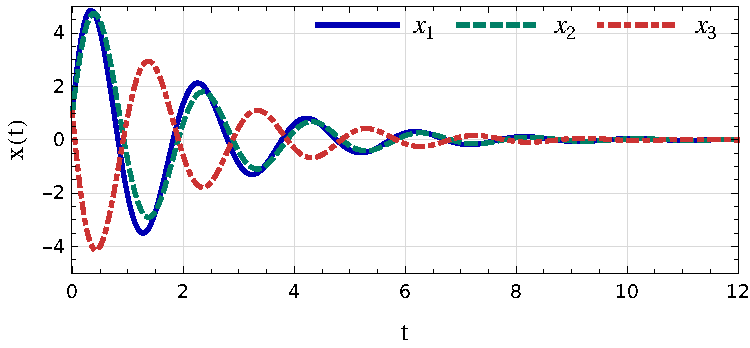
\includegraphics[width=0.7\textwidth]{../images/task1/Xa1K2L.pdf}
		\caption{Вектор состояния $x(t)$ с ограничением на управление}
	\end{figure}
	
	На одном графике построю управление без ограничений на управление \(u_1\) и с ограничением \(u_2\). 
	
	Пунктирными линиями обозначу экспоненциальную огибающую 
	$\pm |u(0)| e^{-\alpha_1 t}$, где $|u(0)|$ — максимальное 
	начальное значение управления. Обе кривые $u_1$ и $u_2$ 
	не выходят за пределы огибающей, что подтверждает затухание 
	управления со степенью устойчивости не менее $\alpha_1 = 0.5$.
	
	\begin{figure}[H]
		\centering
		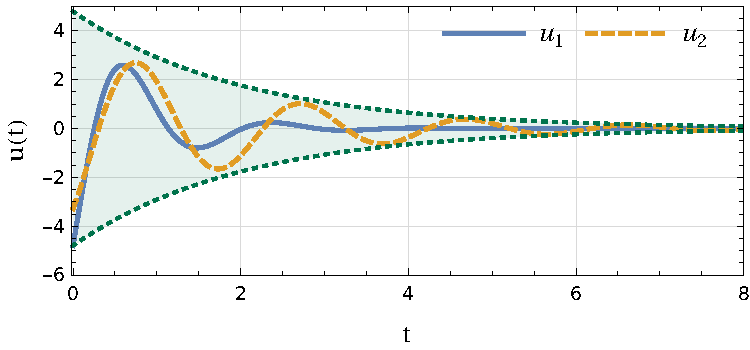
\includegraphics[width=0.7\textwidth]{../images/task1/Ua1L.pdf}
		\caption{Управления \(u(t)\)}
	\end{figure}
	
	\subsubsection{Степень устойчивости $\alpha_2=3$}
	
	Синтезирую регулятор без ограничений на управление. Решу матричное неравенство Ляпунова для усечённой системы:
	\[
	\begin{cases}
		P \hat A_c^T + \hat A_c P + 2\alpha_2 P + Y^T \hat B_c^T + \hat B_c Y \preceq 0 \\
		P \succ 0 \\
		\hat K_\text{1,c} = YP^{-1} \\
	\end{cases}
	\]
	
	Решаю LMI в \texttt{cvx} (листинг~\ref{lst:cvx1}, аналогично). Получаю:
	\[
	\begin{array}{rcl}
		P &=& \begin{bmatrix} 
			2.29 & -3.13\\
			-3.13 & 4.857
		\end{bmatrix} \\[16pt]
		Y &=& \begin{bmatrix} -4.01 & 9.37 \end{bmatrix}
	\end{array}
	\qquad \Longrightarrow \qquad
	\hat{K}_{1,c} = YP^{-1} = \begin{bmatrix} 8.44 & 7.46 \end{bmatrix}
	\]
	
	Дополняю матрицу \(\hat{K}_{1,c}\) нулём для неуправляемого собственного числа и перехожу в исходный базис (листинг~\ref{lst:K1}, аналогично):
	\[
	\hat{K_1} = \begin{bmatrix} 0 & 8.44 & 7.46 \end{bmatrix} 
	\qquad \Longrightarrow \qquad 
	K_1 = \hat{K_1} \cdot P_j^{-1} = \begin{bmatrix} -7.46 & -0.49 & -7.46 \end{bmatrix} 
	\]
	
	Проверяю спектр замкнутой системы (листинг~\ref{lst:lEig1}, аналогично):
	\[
	\sigma(A + BK_1) = \{-4.73 \pm 6.34\mathrm{j},\; -3\}
	\]
	
	Построю графики вектора состояния \(x(t)\) при начальных условиях \(x(0) = \begin{bmatrix} 1 & 1 & 1 \\ \end{bmatrix}^T\) для степени устойчивости \(\alpha_2 = 3\) без ограничений на управление.
	
	\begin{figure}[H]
		\centering
		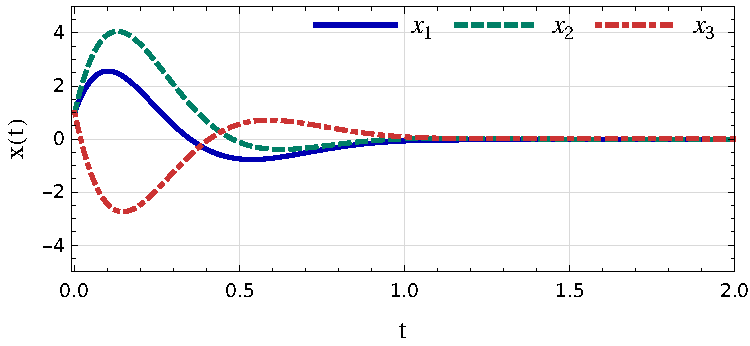
\includegraphics[width=0.7\textwidth]{../images/task1/Xa2K1L.pdf}
		\caption{Вектор состояния $x(t)$ при отсутствии ограничений на управление}
	\end{figure}
	
	Синтезирую регулятор совместно с решением задачи минимизации управления (листинг~\ref{lst:cvxmin1}, аналогично). Получившаяся усеченная матрица регулятора в жордановом базисе:
	\[
	\hat{K}_{2,c} = YP^{-1} = \begin{bmatrix} 5 & 5 \end{bmatrix}
	\]
	
	Перейду в расширенный исходный базис (листинг~\ref{lst:K1}, аналогично):
	\[
	\hat{K_2} = \begin{bmatrix} 0 & 5 & 5 \end{bmatrix} 
	\qquad \Longrightarrow \qquad 
	K_2 = \hat{K_2} \cdot P_j^{-1} = \begin{bmatrix} -5 & 0 & 5 \end{bmatrix} 
	\]
	
	Собственные числа замкнутой системы (листинг~\ref{lst:lEig1}, аналогично):
	\[
	\sigma(A + BK_2) = \{-3 \pm \sqrt{29}\mathrm{j},\; -3\}
	\]
	
	Построю графики вектора состояния \(x(t)\) при начальных условиях \(x(0) = \begin{bmatrix} 1 & 1 & 1 \\ \end{bmatrix}^T\) для степени устойчивости \(\alpha_2 = 3\) с ограничением на управление.
	
	\begin{figure}[H]
		\centering
		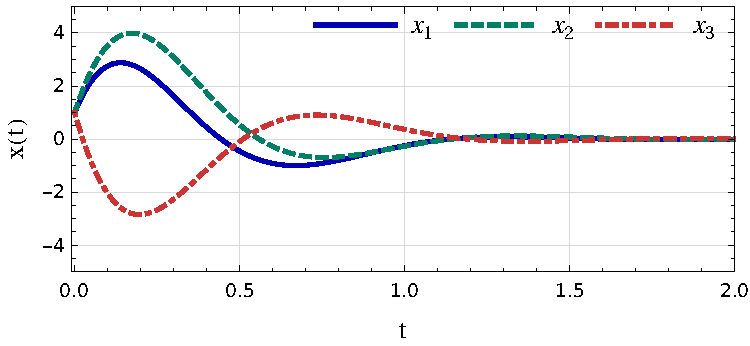
\includegraphics[width=0.7\textwidth]{../images/task1/Xa2K2L.pdf}
		\caption{Вектор состояния $x(t)$ с ограничением на управление}
	\end{figure}
	
	На одном графике построю управление без ограничений на управление \(u_1\) и с ограничением \(u_2\). 
	
	Пунктирными линиями обозначу экспоненциальную огибающую 
	$\pm |u(0)| e^{-\alpha_2 t}$, где $|u(0)|$ — максимальное 
	начальное значение управления. Обе кривые $u_1$ и $u_2$ 
	не выходят за пределы огибающей, что подтверждает затухание 
	управления со степенью устойчивости не менее $\alpha_2 = 3$.
	
	\begin{figure}[H]
		\centering
		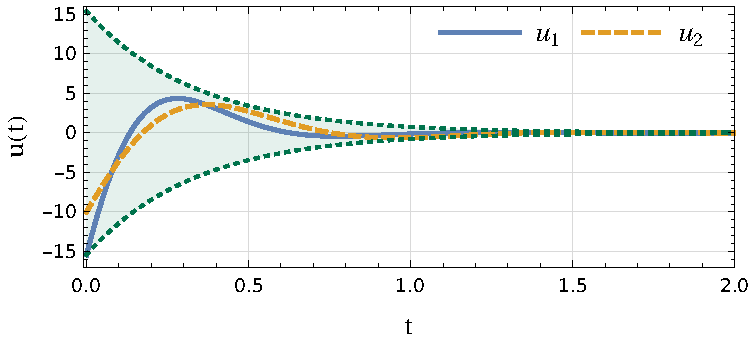
\includegraphics[width=0.7\textwidth]{../images/task1/Ua2L.pdf}
		\caption{Управления \(u(t)\)}
	\end{figure}
	
	\subsection{Синтез регуляторов матричным уравнением типа Риккати}
	
	Синтезирую регуляторы $K_3$, $K_4$ на основе матричного уравнения 
	типа Риккати при $\nu = 2$, $R = 1$:
	\[
	\begin{cases}
		A^\top P + PA + Q - \nu P B R^{-1} B^\top P + 2\alpha P = 0 \\
		K = -R^{-1}B^\top P
	\end{cases}
	\]

	Введя замену $\tilde{A} = A + \alpha I$, перепишу первое уравнение в виде:
	\[
	\tilde{A}^\top P + P\tilde{A} + Q - \nu P B R^{-1} B^\top P = 0
	\]
	
	что эквивалентно решению \texttt{RiccatiSolve[]} с матрицами 
	$\tilde{A}$ и $R/\nu$ (листинг~\ref{lst:riccati1}).
	
	\subsubsection{Степень устойчивости $\alpha_1 = 0.5$}
	
	Решу уравнение Риккати при $Q = I$ (листинг~\ref{lst:riccati1}). Получаю:
	\[
	P = \begin{bmatrix}
	   5.01	& 0.17 & 4.27 \\
	   0.17	& 0.39 & 0.19 \\
	   4.27 & 0.19 & 3.89 \\
	\end{bmatrix}
	\qquad \Longrightarrow \qquad
	K_3 = -R^{-1}B^\top P = \begin{bmatrix} -7.3 & 0.76 & -6.79 \end{bmatrix}
	\]
	
	Проверяю спектр замкнутой системы:
	\[
	\sigma(A + BK_3) = \{-5.67 \pm 3.86\mathrm{j},\; -3\}
	\]
	
	Построю графики вектора состояния \(x(t)\) при начальных условиях \(x(0) = \begin{bmatrix} 1 & 1 & 1 \\ \end{bmatrix}^T\) для степени устойчивости \(\alpha_1 = 0.5\) при \(Q = I\).
	
	\begin{figure}[H]
		\centering
		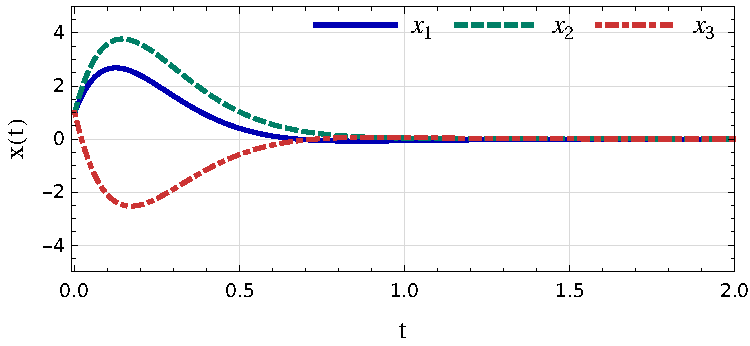
\includegraphics[width=0.7\textwidth]{../images/task1/Xa1Q1R.pdf}
		\caption{Вектор состояния $x(t)$ при \(Q = I\)}
	\end{figure}
	
	Решу уравнение Риккати при $Q = 0$ (листинг~\ref{lst:riccati0}). Получаю:
	\[
	K_4 = -R^{-1}B^\top P = \begin{bmatrix} -3.7 & 0.86 & -3.7 \end{bmatrix}
	\]
	
	Проверяю спектр замкнутой системы:
	\[
	\sigma(A + BK_4) = \{-3 \pm 2\mathrm{j},\; -3\}
	\]
	
	Построю графики вектора состояния \(x(t)\) при начальных условиях \(x(0) = \begin{bmatrix} 1 & 1 & 1 \\ \end{bmatrix}^T\) для степени устойчивости \(\alpha_1 = 0.5\) при \(Q = 0_{3\times3}\).
	
	\begin{figure}[H]
		\centering
		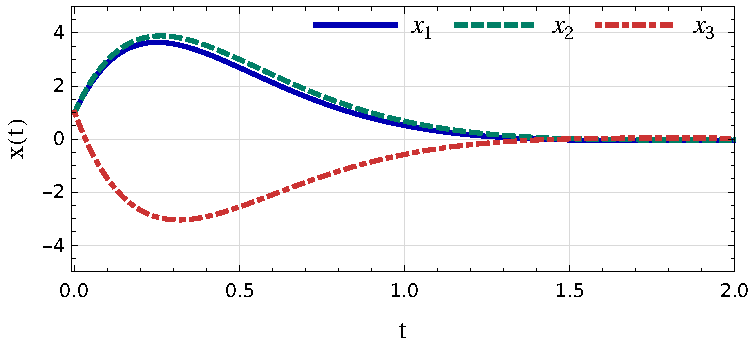
\includegraphics[width=0.7\textwidth]{../images/task1/Xa1Q0R.pdf}
		\caption{Вектор состояния $x(t)$ при \(Q = 0_{3\times3}\)}
	\end{figure}
	
	На одном графике построю управление при \(Q = I\)--- \(u_1\) и при \(Q = 0_{3\times3}\)--- \(u_0\). 
	
	Пунктирными линиями обозначу экспоненциальную огибающую 
	$\pm |u(0)| e^{-\alpha_1 t}$, где $|u(0)|$ — максимальное 
	начальное значение управления. Обе кривые $u_1$ и $u_0$ 
	не выходят за пределы огибающей, что подтверждает затухание 
	управления со степенью устойчивости не менее $\alpha_1 = 0.5$.
	
	\begin{figure}[H]
		\centering
		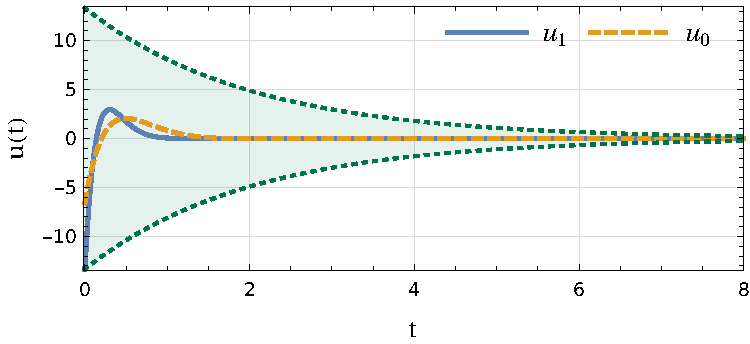
\includegraphics[width=0.7\textwidth]{../images/task1/Ua1R.pdf}
		\caption{Управления \(u(t)\)}
	\end{figure}
\subsubsection{Степень устойчивости $\alpha_2 = 3$}

	При $\alpha_2 = 3$ уравнение Риккати не имеет 
	стабилизирующего решения. Это объясняется тем, что замена 
	$\tilde{A} = A + \alpha_2 I$ сдвигает неуправляемое собственное 
	число $\lambda_1 = -3$ точно в начало координат:
	\[
	\tilde{\lambda}_1 = -3 + 3 = 0
	\]
	после чего система с матрицей $\tilde{A}$ перестаёт быть 
	стабилизируемой. В связи с этим для синтеза регуляторов 
	по методу Риккати я беру $\alpha_2 = 2.9$.
	
	Решу уравнение при $Q = I$ (листинг~\ref{lst:riccati1}, аналогично):
	\[
	K_3 = -R^{-1}B^\top P = \begin{bmatrix} -12.87 & 0.05 & -11.89 \end{bmatrix}
	\]
	Проверяю спектр замкнутой системы:
	\[
	\sigma(A + BK_3) = \{-9.48 \pm 3.72 \mathrm{j},\; -3\}
	\]
	
	Построю графики вектора состояния \(x(t)\) при начальных условиях \(x(0) = \begin{bmatrix} 1 & 1 & 1 \\ \end{bmatrix}^T\) для степени устойчивости \(\alpha_2 = 3\) при \(Q = I\).
	
	\begin{figure}[H]
		\centering
		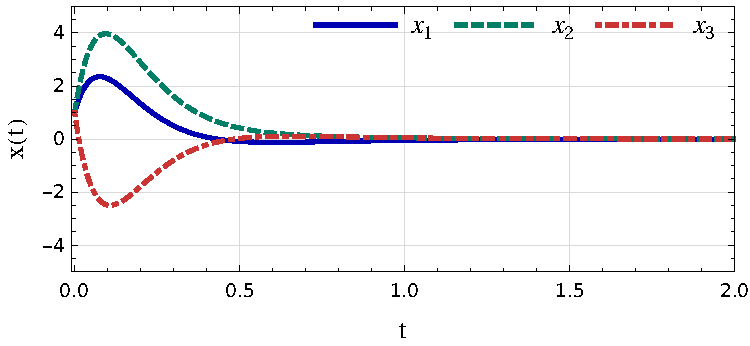
\includegraphics[width=0.7\textwidth]{../images/task1/Xa2Q1R.pdf}
		\caption{Вектор состояния $x(t)$ при \(Q = I\)}
	\end{figure}
	
	Решу уравнение Риккати при $Q = 0$ (листинг~\ref{lst:riccati0}, аналогично). Получаю:
	\[
	P = \begin{bmatrix}
		6.27 & 0.95 & 6.27 \\
		0.95 & 0.65 & 0.95 \\
		6.27 & 0.95 & 6.27
	\end{bmatrix}
	\qquad \Longrightarrow \qquad
	K_4 = -R^{-1}B^\top P = \begin{bmatrix} -9.7 & 0.07 & -9.7 \end{bmatrix}
	\]
	
	Проверяю спектр замкнутой системы:
	\[
	\sigma(A + BK_4) = \{-7.8 \pm 2\mathrm{j},\; -3\}
	\]
	
	Построю графики вектора состояния \(x(t)\) при начальных условиях \(x(0) = \begin{bmatrix} 1 & 1 & 1 \\ \end{bmatrix}^T\) для степени устойчивости \(\alpha_2 = 3\) при \(Q = 0_{3\times3}\).
	
	\begin{figure}[H]
		\centering
		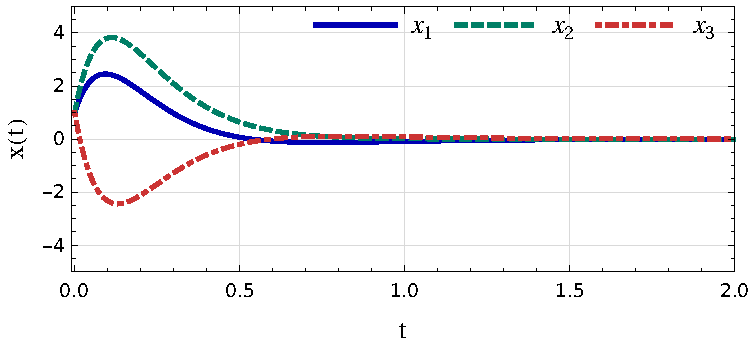
\includegraphics[width=0.7\textwidth]{../images/task1/Xa2Q0R.pdf}
		\caption{Вектор состояния $x(t)$ при \(Q = 0_{3\times3}\)}
	\end{figure}
	
	На одном графике построю управление при \(Q = I\)--- \(u_1\) и при \(Q = 0_{3\times3}\)--- \(u_0\). 
	
	Пунктирными линиями обозначу экспоненциальную огибающую 
	$\pm |u(0)| e^{-\alpha_2 t}$, где $|u(0)|$ — максимальное 
	начальное значение управления. Обе кривые $u_1$ и $u_0$ 
	не выходят за пределы огибающей, что подтверждает затухание 
	управления со степенью устойчивости не менее $\alpha_2 = 3$.
	
	\begin{figure}[H]
		\centering
		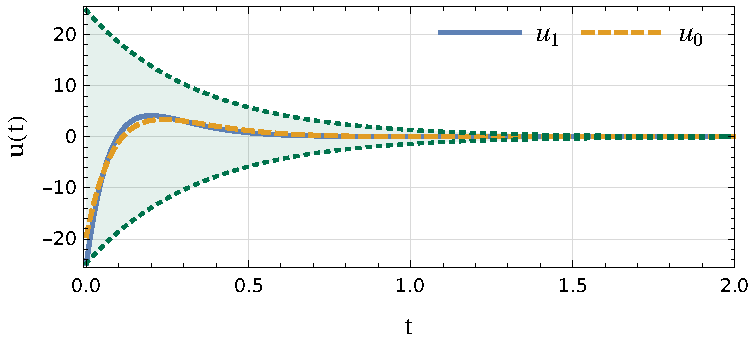
\includegraphics[width=0.7\textwidth]{../images/task1/Ua2R.pdf}
		\caption{Управления \(u(t)\)}
	\end{figure}
	
	\newpage \subsection{Вывод по заданию}
	
	Сравню спектры всех четырёх регуляторов для каждой степени устойчивости.
	
	Все регуляторы обеспечивают заданную степень устойчивости ---
	вещественные части управляемых собственных чисел не превышают 
	$-\alpha$ по модулю. Неуправляемое собственное число 
	$\lambda_1 = -3$ остаётся фиксированным во всех случаях.
	
	Регуляторы по методу Риккати ($K_3$, $K_4$) располагают 
	собственные числа значительно левее требуемой границы по 
	сравнению с регуляторами Ляпунова ($K_1$, $K_2$), что 
	соответствует более быстрому затуханию, но и большим 
	начальным значениям управления. При $Q = 0$ регулятор $K_4$ 
	даёт меньшее управляющее воздействие, чем $K_3$ при $Q = I$, 
	поскольку матрица $Q = 0$.
	
	\newpage \section{Управление по выходу с заданной степенью устойчивости}
	
	В соответствии с вариантом рассмотрю систему:
	\[
	\begin{cases}
		\dot{x} = Ax + Bu \\
		y = Cx
	\end{cases}
	\]
	
	\[
	A = \begin{bmatrix}
		5 & -9 & -7 & 1 \\
		-9 & 5 & -1 & 7 \\
		-7 & -1 & 5 & 9 \\
		1 & 7 & 9 & 5
	\end{bmatrix} \qquad
	B = \begin{bmatrix} 3 \\ 3 \\ 1 \\ 3 \end{bmatrix}  \qquad
	C = \begin{bmatrix} 2 & -2 & 2 & 2 \\ -2 & 4 & 2 & 4 \end{bmatrix}
	\]
	
	Требуется:
	
	\begin{enumerate}
		\item Найти собственные числа матрицы $A$ и определить управляемость
		и наблюдаемость каждого из них. Сделать вывод об управляемости,
		стабилизируемости, наблюдаемости и обнаруживаемости системы.
		
		\item Определить достижимую степень устойчивости при регуляторе $u = Kx$
		и максимальную степень сходимости наблюдателя.
		
		\item Построить схему моделирования системы, замкнутой наблюдателем
		и регулятором.
		
		\item Задаться несколькими значениями $\alpha > 0$ и составить не менее
		трёх наборов $(\alpha_K,\, \alpha_L)$, охватывающих случаи
		$\alpha_K = \alpha_L$, $\alpha_K > \alpha_L$ и $\alpha_K < \alpha_L$.
		
		\item Для каждого набора синтезировать регулятор $K$ и наблюдатель $L$,
		проверить спектры $(A + BK)$ и $(A + LC)$, выполнить моделирование.
		
		\item Сравнить результаты и сделать выводы.
	\end{enumerate}
	
	\hrule \newpage
	
	\subsection{Анализ матрицы системы}
	
	Найду собственные числа матрицы \(A\):
	\[
	\operatorname{det}(\lambda I - A) = \operatorname{det}\begin{bmatrix}
		\lambda-5 & 9 & 7 & -1 \\
		9 & \lambda-5 & 1 & -7 \\
		7 & 1 & \lambda-5 & -9 \\
		-1 & -7 & -9 & \lambda-5 \\
	\end{bmatrix} = \lambda^4 - 20\lambda^3 - 112\lambda^2 + 960\lambda + 7680 = 0
	\]
	
	\[
	\sigma(A) = \{20,\; -12,\; 8,\; 4\}
	\]
	
	Собственные числа матрицы вещественные и различные, значит будет легко перейти в жорданов базис. Переведу всю систему в жорданов базис (листинг~\ref{lst:jordan2}):
	\[
	\begin{cases}
		\dot{\hat x} =
		\begin{bmatrix}
			-12 & 0 & 0 & 0 \\
			0 & 4 & 0 & 0 \\
			0 & 0 & 8 & 0 \\
			0 & 0 & 0 & 20
		\end{bmatrix}
		\hat x
		+ \begin{bmatrix}
			-1 \\ 2 \\ 1 \\ 1 \\
		\end{bmatrix} u
		\\[30pt]
		y = 
		\begin{bmatrix}
			0 & 0 & 8 & 0 \\
			0 & 4 & 0 & 12 \\
		\end{bmatrix}
		\hat x
	\end{cases}
	\]
	
Все компоненты матрицы \(\hat B\) ненулевые, следовательно, все собственные числа матрицы системы управляемы.

Первый столбец матрицы \(\hat C\) нулевой, значит соответствующее ему собственное число \(-12\) ненаблюдаемо. Остальные собственные числа наблюдаемы, так как им соответствуют ненулевые столбцы матрицы \(\hat C\).

Система является полностью управляемой и не полностью наблюдаемой.

Система является стабилизируемой, так как все неустойчивые собственные числа \(\{4,\; 8,\; 20\}\) управляемы.

Система является обнаруживаемой, так как все неустойчивые собственные числа наблюдаемы, а ненаблюдаемое собственное число устойчиво.
	
	\subsection{Максимальные степени устойчивости и сходимости}
	
	Так как система полностью управляема, то можно добиться любой степени устойчивости при помощи регулятора вида \(u = K x\).
	
	Так как система не полностью наблюдаема, то нельзя добиться любой желаемой степени сходимости наблюдателя. Максимальная достижимая степень сходимости ограничена этой ненаблюдаемой модой и равна \(12\). 
	
	Составлю следующие наборы для синтеза:
	
	\begin{enumerate}
		\item \(\alpha_K = \alpha_L = 10\) — регулятор и наблюдатель имеют сопоставимую динамику;
		\item \(\alpha_K = 12,\ \alpha_L = 4\) — регулятор существенно сильнее наблюдателя;
		\item \(\alpha_K = 4,\ \alpha_L = 10\) — наблюдатель существенно сильнее регулятора.
	\end{enumerate}
	
	
	\subsection{Структурная схема системы}

	Введу ошибку наблюдателя $e = \hat{x} - x$. Тогда:
	\[
	\dot{e} = \dot{\hat{x}} - \dot{x} 
	= \bigl[(A + BK)\hat{x} + LC(\hat{x} - x)\bigr] - \bigl[Ax + BK\hat{x}\bigr]
	= A(\hat{x} - x) + LC(\hat{x} - x)
	= (A + LC)e
	\]
	
	Подставлю $\hat{x} = x + e$ в уравнение системы:
	\[
	\dot{x} = Ax + BK\hat{x} = Ax + BK(x + e) = (A + BK)x + BKe
	\]
	
	Исходная система принимает вид:
	\[
	\begin{cases}
		\dot{x} = (A + BK)x + BKe \\
		\dot{e} = (A + LC)e
	\end{cases}
	\]

	Построю схему системы. 
	
\begin{figure}[H]
	\centering
	\begin{tikzpicture}[
		block/.style={draw, rectangle, minimum width=2.5cm, minimum height=0.9cm,
			align=center, fill=blue!8, rounded corners=2pt, thick},
		intblock/.style={draw, rectangle, minimum width=0.8cm, minimum height=0.8cm,
			align=center, fill=orange!15, rounded corners=2pt, thick},
		sumblock/.style={draw, rectangle, minimum width=0.8cm, minimum height=0.8cm,
			align=center, fill=green!10, rounded corners=2pt, thick},
		arrow/.style={-{Stealth[length=2mm]}, thick},
		]
		
		%% ── ВЕРХНИЙ КОНТУР ─────────────────────────────────────
		\node[block]    (ABK)  at (0, 0)    {$A + BK$};
		\node[sumblock] (sumX) at (2.4, 0) {$+$\\$+$};
		\node[intblock] (intX) at (3.8, 0)  {$\dfrac{1}{s}$};
		
		\draw[arrow] (ABK)  -- (sumX);
		\draw[arrow] (sumX) -- node[above]{\small$\dot{x}$} (intX);
		
		% x
		\coordinate (xbr) at ($(intX.east)+(0.6,0)$);
		\draw[thick] (intX.east) -- (xbr);
		\node[above right=-1.5cm and -2cm of xbr] {$x$};
		
		% опущенная обратная связь x
		\coordinate (xdown) at ($(xbr)+(0,-1.5)$);
		\draw[arrow] (xbr) -- (xdown) -| (ABK.south);
		
		% BK сверху
		\node[block, minimum width=1.4cm] (BKb) at (2.4, 1.9) {$BK$};
		\draw[arrow] (BKb) -- (sumX.north);
		
		%% ── ПРАВЫЙ КОНТУР (e) ───────────────────────────────────
		\node[block]    (ALC)  at (7, 0)   {$A + LC$};
		\node[intblock] (intE) at (10.8, 0) {$\dfrac{1}{s}$};
		
		\draw[arrow] (ALC) -- node[above]{\small$\dot{e}$} (intE);
		
		% e
		\coordinate (ebr) at ($(intE.east)+(0.6,0)$);
		\draw[thick] (intE.east) -- (ebr);
		\node[above right=-1.5cm and 4.3cm of xbr] {$e$};
		
		% опущенная обратная связь e
		\coordinate (edown) at ($(ebr)+(0,-1.5)$);
		\draw[arrow] (ebr) -- (edown) -| (ALC.south);
		
		%% ── СВЯЗЬ e → BK ───────────────────────────────────────
		\draw[arrow] (ebr) |- (BKb.east);
		
	\end{tikzpicture}
	\caption{Структурная схема системы}
\end{figure}
	
	\subsection{Набор 1: $\alpha_K = \alpha_L = 10$}
	
	Для этого набора наблюдатель и регулятор имеют сопоставимые значения \(\alpha\).
	
	\subsubsection{Синтез регулятора \(K_1\)}

	Для обеспечения степени устойчивости $\alpha_K = 10$ решу уравнение Риккати с заменой:
	\[
	\begin{cases}
		\tilde{A}^\top P + P\tilde{A} + Q - \nu P B R^{-1} B^\top P = 0 \\
		\tilde{A} = A + \alpha_K I \\
		K_1 = -R^{-1}B^\top P
	\end{cases}
	\]
	
	Приму весовые матрицы следующими: $Q = I_{4\times4}$, $R = 1$, $\nu = 1$. Решую уравнение Риккати (листинг~\ref{lst:K21}):
	\[\begin{aligned}
		P &= \begin{bmatrix}
			3294.86 & -5028.83 & 2508.28 & 766.32 \\
			-5028.83 & 7734.28 & -3928.21 & -1209.42 \\
			2508.28 & -3928.21 & 2082.19 & 653.62 \\
			766.32 & -1209.41 & 653.62 & 208.19
		\end{bmatrix} \\[5pt]
		K_1 &= \begin{bmatrix} 394.67 & -559.91 & 216.74 & 51.11 \end{bmatrix}
	\end{aligned}
	\]
	
	Спектр замкнутой системы:
	\[
	\sigma(A + BK_1) = \{-42.17,\; -25.40 \pm 3.95\mathrm{j},\; -12.68\}
	\]
	
	Минимальная по модулю вещественная часть равна $12.68$, что превышает требуемую степень устойчивости $\alpha_K = 10$. Синтез выполнен корректно.
	
	\subsubsection{Синтез наблюдателя $L_1$}
	
	Для обеспечения заданной степени сходимости $\alpha_L = 10$ синтезирую наблюдатель на основе матричного неравенства Ляпунова для наблюдаемой части системы в жордановом базисе:
	\[
	\hat A_c =
	\begin{bmatrix}
		4 & 0 & 0 \\
		0 & 8 & 0 \\
		0 & 0 & 20
	\end{bmatrix} \qquad
	\hat C_c =
	\begin{bmatrix}
		0 & 8 & 0 \\
		4 & 0 & 12
	\end{bmatrix}
	\]
	
	Решу матричное неравенство (листинг~\ref{lst:L21}):
	\[
	\begin{cases}
		\hat A_c Q + Q \hat A_c^\top + 2\alpha_L Q + Y \hat C_c + \hat C_c^\top Y^\top \preceq 0 \\
		Q \succ 0
	\end{cases}
	\]
	
	И найду матрицу наблюдателя:
	\[
	\hat L_c = Q^{-1} Y
	\]
	
	Полученную матрицу $\hat L_c$ расширяю до полной размерности, добавляя нулевую строку, соответствующую ненаблюдаемой моде, и выполняю переход в исходный базис:
	\[
	L_1 = P \hat L
	\]

	Запишу матрицу наблюдателя \(L_1\) в исходном базисе:
	\[
	L_1 = \begin{bmatrix}
		-2.3 & 14.13 \\
		2.3 & 1.38 \\
		-2.3 & -14.13 \\
		-2.3 & 1.38 \\
	\end{bmatrix}
	\]
	
	Проверяю спектр матрицы замкнутой системы:
	\[
	\sigma(A + L_1 C) =
	\left\{
	-10.74 \pm 16.70\,\mathrm{j},\;
	-12,\;
	-10.40
	\right\}
	\]
	
	Вещественные части собственных чисел отрицательны, система устойчива.
	
	\subsubsection{Моделирование}
	
	Графики управления, сравнения состояний и ошибки наблюдения приведены ниже.
	
	\begin{figure}[H]
		\centering
		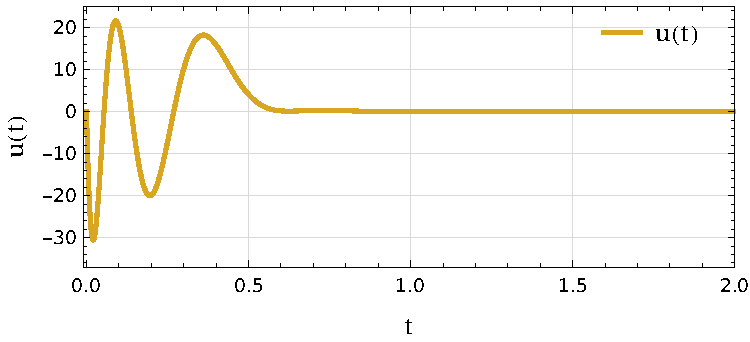
\includegraphics[width=0.7\textwidth]{../images/task2/U1.pdf}
		\caption{Управление \(u(t)\)}
	\end{figure}
	
	
	\begin{figure}[H]
		\centering
		\begin{minipage}{0.48\textwidth}
			\centering
			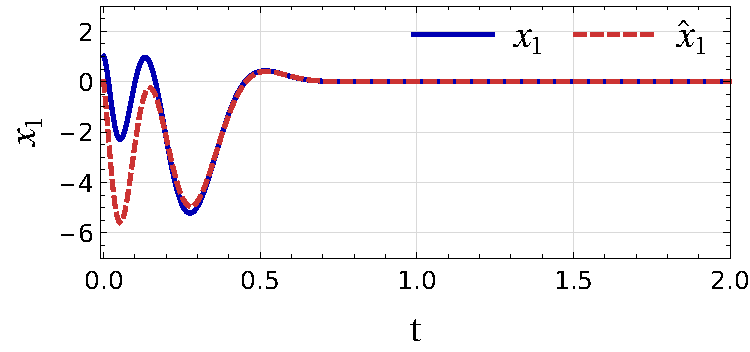
\includegraphics[width=\textwidth]{../images/task2/xx11.pdf}
			\caption{\(x_1(t)\) и \(\hat{x}_1(t)\)}
		\end{minipage}
		\hfill
		\begin{minipage}{0.48\textwidth}
			\centering
			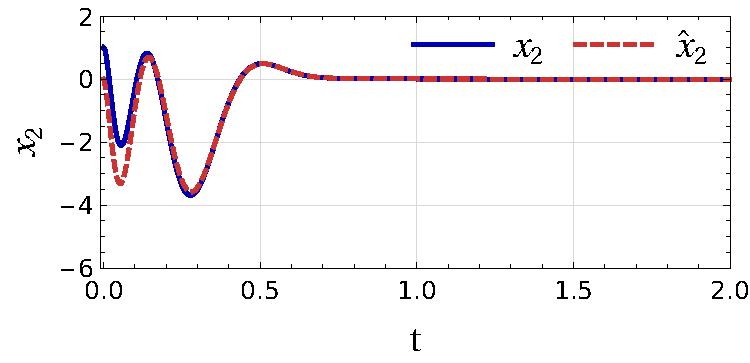
\includegraphics[width=\textwidth]{../images/task2/xx12.pdf}
			\caption{\(x_2(t)\) и \(\hat{x}_2(t)\)}
		\end{minipage}
		
		\vspace{0.5cm}
		
		\begin{minipage}{0.48\textwidth}
			\centering
			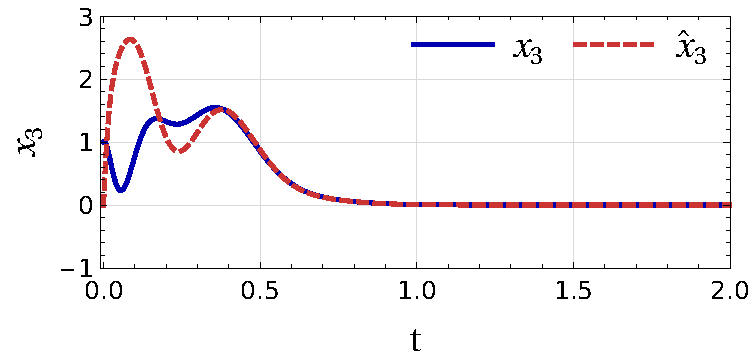
\includegraphics[width=\textwidth]{../images/task2/xx13.pdf}
			\caption{\(x_3(t)\) и \(\hat{x}_3(t)\)}
		\end{minipage}
		\hfill
		\begin{minipage}{0.48\textwidth}
			\centering
			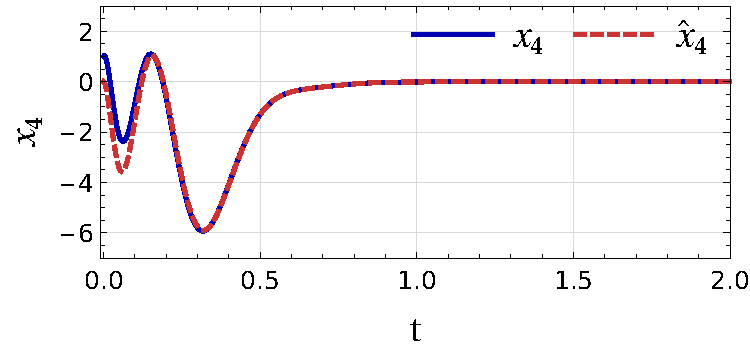
\includegraphics[width=\textwidth]{../images/task2/xx14.pdf}
			\caption{\(x_4(t)\) и \(\hat{x}_4(t)\)}
		\end{minipage}
	\end{figure}
	
	
	\begin{figure}[H]
		\centering
		
\includegraphics[width=0.7\textwidth]{../images/task2/e1.pdf}
		\caption{Ошибка \(e(t)\)}
	\end{figure}
	
	По графикам видно, что управление и ошибка наблюдения затухают за \(t \approx 0.6\) секунды. Оценки состояния \(\hat{x}(t)\) быстро сходятся к истинным значениям \(x(t)\). Это соответствует заданной степени устойчивости \(\alpha_K = \alpha_L  = 10\).
	
	\subsection{Набор 2: $\alpha_K = 12, \alpha_L = 4$}
	
	Для этого набора регулятор сильнее наблюдателя.
	
	\subsubsection{Синтез регулятора \(K_2\)}
	
	Для обеспечения степени устойчивости $\alpha_K = 4$ решу уравнение Риккати с заменой:
	\[
	\begin{cases}
		\tilde{A}^\top P + P\tilde{A} + Q - \nu P B R^{-1} B^\top P = 0 \\
		\tilde{A} = A + \alpha_K I \\
		K_2 = -R^{-1}B^\top P
	\end{cases}
	\]
	
	Приму весовые матрицы такими же, как и для первого набора: $Q = I_{4\times4}$, $R = 1$, $\nu = 1$. Решую уравнение Риккати (листинг~\ref{lst:K21}, аналогично):
		\[\begin{aligned}
		P &= \begin{bmatrix}
			5616.97 & -8782.54 & 4646.58 & 1438.16 \\
			-8782.53 & 13820.8 & -7416.06 & -2305.75 \\
			4646.58 & -7416.06 & 4104.68 & 1289.43 \\
			1438.16 & -2305.71 & 1289.43 & 408.53
		\end{bmatrix} \\[5pt]
		K_2 &= \begin{bmatrix} 535.62 & -781.47 & 335.47 & 87.75 \end{bmatrix}
	\end{aligned}
	\]
	
	Спектр замкнутой системы:
	\[
	\sigma(A + BK_2) = \{-47.85,\; -28.63 \pm 5.98\,\mathrm{j} ,\; -13.71\}
	\]
	
	Минимальная по модулю вещественная часть равна $13.71$, что превышает требуемую степень устойчивости $\alpha_K = 12$. Синтез выполнен корректно.
	
	\subsubsection{Синтез наблюдателя $L_2$}
	
	Для обеспечения заданной степени сходимости $\alpha_L = 12$ синтезирую наблюдатель на основе матричного неравенства Ляпунова для наблюдаемой части системы в жордановом базисе:
	\[
	\hat A_c =
	\begin{bmatrix}
		4 & 0 & 0 \\
		0 & 8 & 0 \\
		0 & 0 & 20
	\end{bmatrix} \qquad
	\hat C_c =
	\begin{bmatrix}
		0 & 8 & 0 \\
		4 & 0 & 12
	\end{bmatrix}
	\]
	
	Решу матричное неравенство (листинг~\ref{lst:L21}, аналогично):
	\[
	\begin{cases}
		\hat A_c Q + Q \hat A_c^\top + 2\alpha_L Q + Y \hat C_c + \hat C_c^\top Y^\top \preceq 0 \\
		Q \succ 0
	\end{cases}
	\]
	
	И найду матрицу наблюдателя:
	\[
	\hat L_c = Q^{-1} Y
	\]
	
	Полученную матрицу $\hat L_c$ расширяю до полной размерности, добавляя нулевую строку, соответствующую ненаблюдаемой моде, и выполняю переход в исходный базис:
	\[
	L_2 = P \hat L
	\]
	
	Запишу матрицу наблюдателя \(L_2\) в исходном базисе:
	\[
	L_2 = \begin{bmatrix}
		-1.55 & 6.85 \\
		1.55 & -0.73 \\
		-1.55 & -6.85 \\
		-1.55 & -0.73
	\end{bmatrix}	
	\]
	
	Проверяю спектр матрицы замкнутой системы:
	\[
	\sigma(A + L_2 C) = \{-12,\; -4.62 \pm 11.02\,\mathrm{j},\; -4.4\}
	\]
	
	Вещественные части собственных чисел отрицательны, система устойчива.
	
	
	\subsubsection{Моделирование}
	
	Графики управления, сравнения состояний и ошибки наблюдения приведены ниже.
	
	\begin{figure}[H]
		\centering
		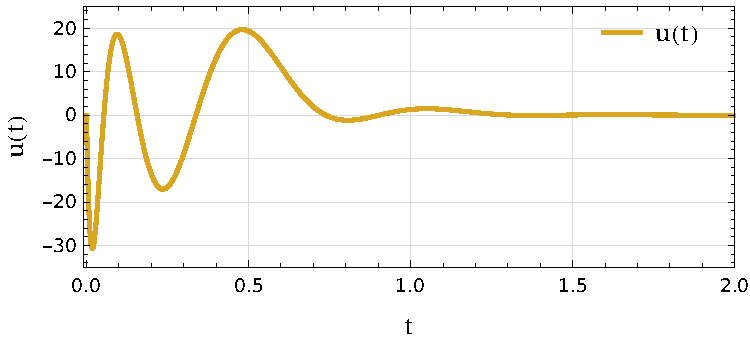
\includegraphics[width=0.7\textwidth]{../images/task2/U2.pdf}
		\caption{Управление \(u(t)\)}
	\end{figure}
	
	
	\begin{figure}[H]
		\centering
		\begin{minipage}{0.48\textwidth}
			\centering
			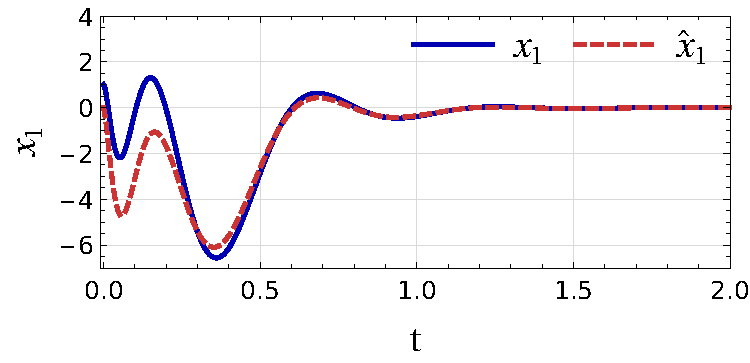
\includegraphics[width=\textwidth]{../images/task2/xx21.pdf}
			\caption{\(x_1(t)\) и \(\hat{x}_1(t)\)}
		\end{minipage}
		\hfill
		\begin{minipage}{0.48\textwidth}
			\centering
			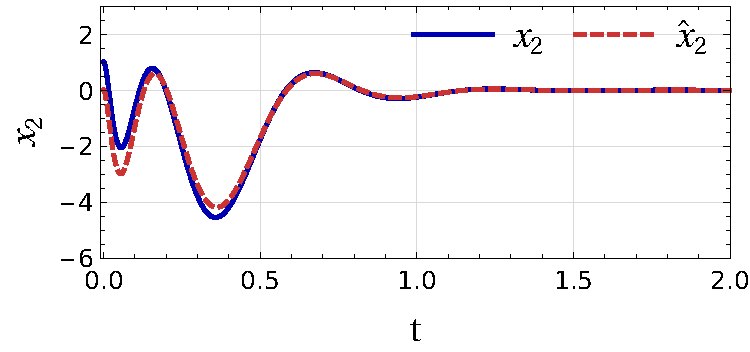
\includegraphics[width=\textwidth]{../images/task2/xx22.pdf}
			\caption{\(x_2(t)\) и \(\hat{x}_2(t)\)}
		\end{minipage}
		
		\vspace{0.5cm}
		
		\begin{minipage}{0.48\textwidth}
			\centering
			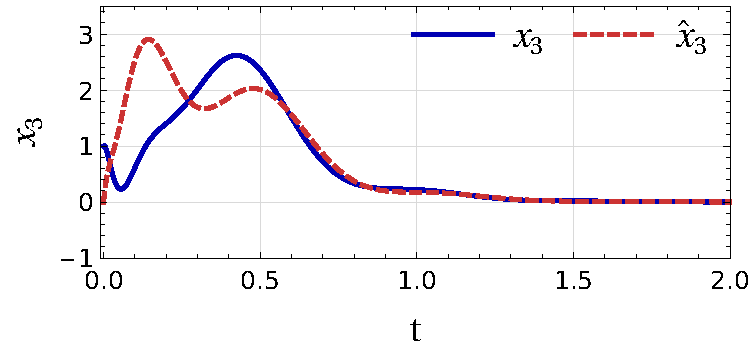
\includegraphics[width=\textwidth]{../images/task2/xx23.pdf}
			\caption{\(x_3(t)\) и \(\hat{x}_3(t)\)}
		\end{minipage}
		\hfill
		\begin{minipage}{0.48\textwidth}
			\centering
			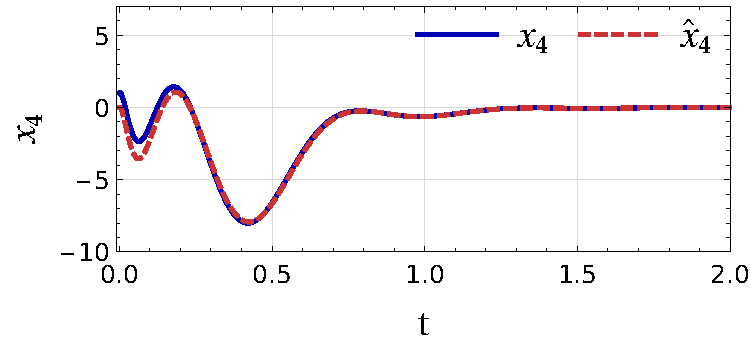
\includegraphics[width=\textwidth]{../images/task2/xx24.pdf}
			\caption{\(x_4(t)\) и \(\hat{x}_4(t)\)}
		\end{minipage}
	\end{figure}
	
	
	\begin{figure}[H]
		\centering
		
\includegraphics[width=0.7\textwidth]{../images/task2/e2.pdf}
		\caption{Ошибка \(e(t)\)}
	\end{figure}
	
	По графикам видно, что управление затухает за \(t \approx 1\) секунду. Оценки состояния \(\hat{x}(t)\) быстро сходятся к истинным значениям \(x(t)\). Это соответствует заданной степени устойчивости \(\alpha_K = 12\), \(\alpha_L = 4\).
	
	По сравнению с первым набором, графики имеют ту же форму, но наблюдатель чуть дольше догоняет регулятор. Это связано с тем, что большое \(\alpha_K\) требует более сильного управления. Наблюдатель с \(\alpha_L = 4\) работает медленнее, но всё равно справляется.
	
	
	\subsection{Набор 3: $\alpha_K = 4, \alpha_L = 12$}
	
	Для этого набора наблюдатель сильнее регулятора.
	
	\subsubsection{Синтез регулятора \(K_3\)}
	
	Для обеспечения степени устойчивости $\alpha_K = 12$ решу уравнение Риккати с заменой:
	\[
	\begin{cases}
		\tilde{A}^\top P + P\tilde{A} + Q - \nu P B R^{-1} B^\top P = 0 \\
		\tilde{A} = A + \alpha_K I \\
		K_3 = -R^{-1}B^\top P
	\end{cases}
	\]
	
	Приму весовые матрицы такими же, как и для первого набора: $Q = I_{4\times4}$, $R = 1$, $\nu = 1$. Решую уравнение Риккати (листинг~\ref{lst:K21}, аналогично):
	\[\begin{aligned}
		P &= \begin{bmatrix}
			621.17 & -871.94 & 338.83 & 88.03 \\
			-871.94 & 1239.82 & -503.63 & -135.78 \\
			338.83 & -503.63 & 236.62 & 71.73 \\
			88.03 & -135.78 & 71.73 & 24.07
		\end{bmatrix} \\[5pt]
		K_3 &= \begin{bmatrix} 149.39 & -192.67 & 42.59 & -0.69 \end{bmatrix}
	\end{aligned}
	\]
	
	Спектр замкнутой системы:
	\[
	\sigma(A + BK_3) = \{-27.23,\; -17.86,\; -12.23,\; -12\}
	\]
	
	Минимальная по модулю вещественная часть равна $12$, что значительно превышает требуемую степень устойчивости $\alpha_K = 4$. Синтез выполнен корректно.
	
	\subsubsection{Синтез наблюдателя $L_3$}
	
	Для обеспечения заданной степени сходимости $\alpha_L = 12$ синтезирую наблюдатель на основе матричного неравенства Ляпунова для наблюдаемой части системы в жордановом базисе:
	\[
	\hat A_c =
	\begin{bmatrix}
		4 & 0 & 0 \\
		0 & 8 & 0 \\
		0 & 0 & 20
	\end{bmatrix} \qquad
	\hat C_c =
	\begin{bmatrix}
		0 & 8 & 0 \\
		4 & 0 & 12
	\end{bmatrix}
	\]
	
	Решу матричное неравенство (листинг~\ref{lst:L21}, аналогично):
	\[
	\begin{cases}
		\hat A_c Q + Q \hat A_c^\top + 2\alpha_L Q + Y \hat C_c + \hat C_c^\top Y^\top \preceq 0 \\
		Q \succ 0
	\end{cases}
	\]
	
	И найду матрицу наблюдателя:
	\[
	\hat L_c = Q^{-1} Y
	\]
	
	Полученную матрицу $\hat L_c$ расширяю до полной размерности, добавляя нулевую строку, соответствующую ненаблюдаемой моде, и выполняю переход в исходный базис:
	\[
	L_3 = P \hat L
	\]
	
	Запишу матрицу наблюдателя \(L_3\) в исходном базисе:
	\[
	L_3 = \begin{bmatrix}
		-2.55 & 17.25 \\
		2.55 & 2.43 \\
		-2.55 & -17.25 \\
		-2.55 & 2.43
	\end{bmatrix}	
	\]
	
	Проверяю спектр матрицы замкнутой системы:
	\[
	\sigma(A + L_3 C) = \{-12,\; -12.78 \pm 18.66\,\mathrm{j},\; -12.4\}
	\]
	
	Вещественные части собственных чисел отрицательны, система устойчива.
	
	
	\subsubsection{Моделирование}
	
	Графики управления, сравнения состояний и ошибки наблюдения приведены ниже.
	
	\begin{figure}[H]
		\centering
		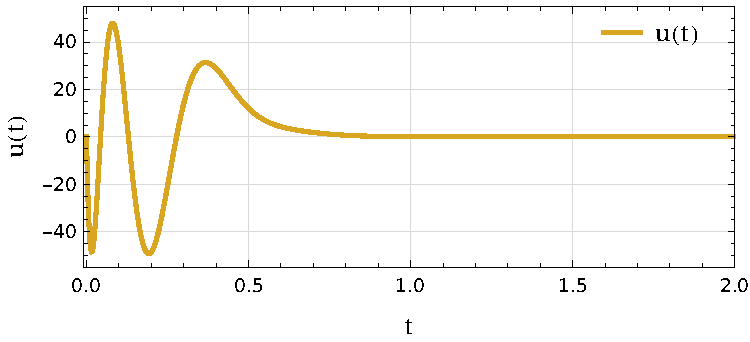
\includegraphics[width=0.7\textwidth]{../images/task2/U3.pdf}
		\caption{Управление \(u(t)\)}
	\end{figure}
	
	
	\begin{figure}[H]
		\centering
		\begin{minipage}{0.48\textwidth}
			\centering
			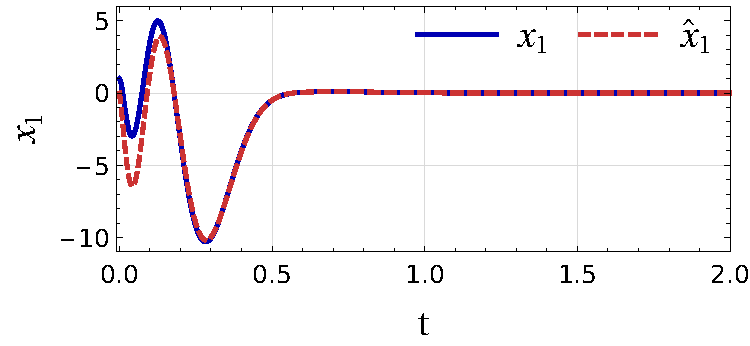
\includegraphics[width=\textwidth]{../images/task2/xx31.pdf}
			\caption{\(x_1(t)\) и \(\hat{x}_1(t)\)}
		\end{minipage}
		\hfill
		\begin{minipage}{0.48\textwidth}
			\centering
			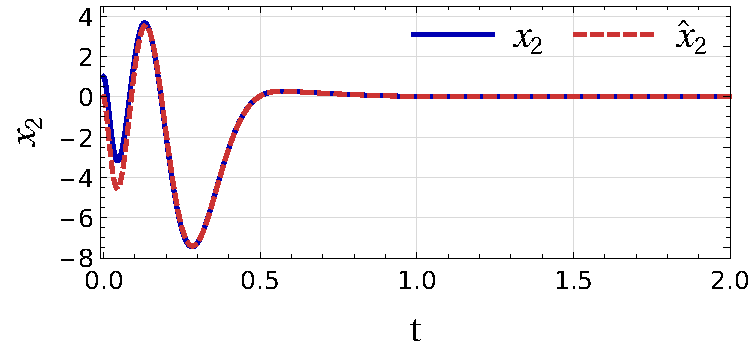
\includegraphics[width=\textwidth]{../images/task2/xx32.pdf}
			\caption{\(x_2(t)\) и \(\hat{x}_2(t)\)}
		\end{minipage}
		
		\vspace{0.5cm}
		
		\begin{minipage}{0.48\textwidth}
			\centering
			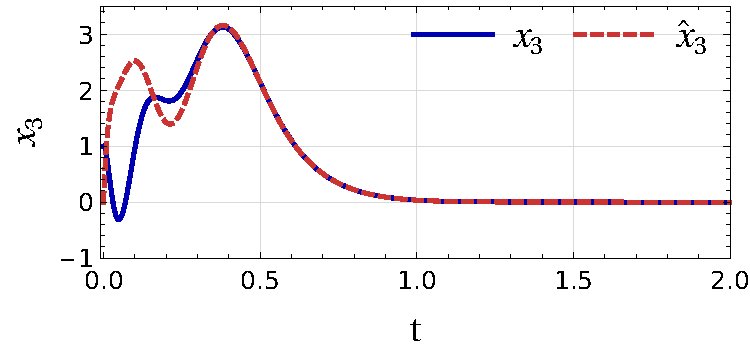
\includegraphics[width=\textwidth]{../images/task2/xx33.pdf}
			\caption{\(x_3(t)\) и \(\hat{x}_3(t)\)}
		\end{minipage}
		\hfill
		\begin{minipage}{0.48\textwidth}
			\centering
			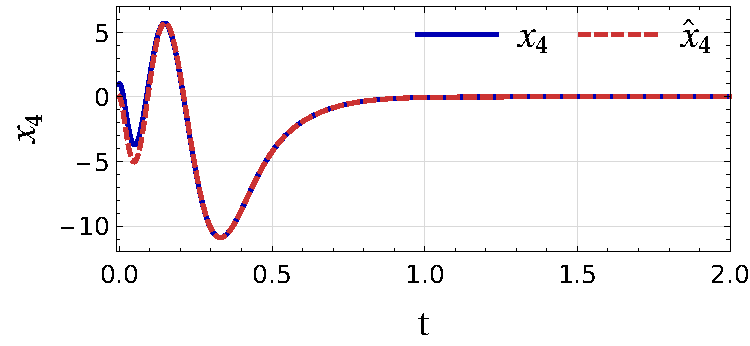
\includegraphics[width=\textwidth]{../images/task2/xx34.pdf}
			\caption{\(x_4(t)\) и \(\hat{x}_4(t)\)}
		\end{minipage}
	\end{figure}
	
	
	\begin{figure}[H]
		\centering
		
\includegraphics[width=0.7\textwidth]{../images/task2/e3.pdf}
		\caption{Ошибка \(e(t)\)}
	\end{figure}
	
	По графикам видно, что управление затухает за \(t \approx 0.7\) секунды. Оценки состояния \(\hat{x}(t)\) быстрее, чем во 2 наборе сходятся к истинным значениям \(x(t)\). Это соответствует заданной степени устойчивости \(\alpha_K = 4\), \(\alpha_L = 12\).
	
	По сравнению с первым набором, графики схожую форму, но вытянуты по оси ординат. Наблюдатель с \(\alpha_L = 12\) работает быстрее, ошибки невязки пропадают за \(t \approx 0.4\) секунды.
	
	 \subsection{Вывод по заданию}
	
	В задании я рассмотрела три случая: $\alpha_K = \alpha_L$, $\alpha_K > \alpha_L$ и $\alpha_K < \alpha_L$. При $\alpha_K > \alpha_L$ управление получается более сильным, но наблюдатель восстанавливает состояние медленнее. При $\alpha_K < \alpha_L$ наблюдатель быстро сходится, однако переходный процесс по выходу затягивается из‑за более слабого регулятора. Наиболее равномерное поведение даёт случай $\alpha_K = \alpha_L$, когда скорости затухания управления и ошибки наблюдения близки. 
	
	\newpage \section{Регулятор с качественной экспоненциальной устойчивостью}
	
	В соответствии с вариантом рассмотрю систему:
	\[
	\dot{x} = Ax + Bu,\qquad 
	A = \begin{bmatrix}
		8 & 1 & 11 \\
		4 & 0 & 4 \\
		-4 & -3 & -7
	\end{bmatrix} \qquad 
	B = \begin{bmatrix}
		-1 \\ -3 \\ 3
	\end{bmatrix}
	\]
	Требуется:
	
	\begin{enumerate}
		\item Найти собственные числа $A$ и определить управляемость.
		
		\item Выбрать параметры $\beta < 0$ и $r > 0$ так, чтобы $\beta + r < 0$, $r = |\beta|/k$ при $1.5 \leq k \leq 4$, а неуправляемые собственные числа попали в круг с центром $(\beta, 0)$ и радиусом $r$.
		
		\item Для четырёх наборов $(Q, R)$: $(I, 1)$, $(I, 0)$, $(0, 1)$, $(0, 0)$ решить уравнение Риккати:
		\[
		\begin{cases}
			(A - BK - \beta I)^\top P (A - BK - \beta I) - r^2 P = -Q \\[8pt]
			K = -(R + B^\top P B)^{-1} B^\top P (A - \beta I)
		\end{cases}
		\]
		
		\item Для каждого набора:
		\begin{enumerate}
			\item[a)] найти $K$;
			\item[б)] проверить, что собственные числа $A+BK$ лежат внутри круга;
			\item[в)] построить графики $u(t)$ и $x(t)$ при $x(0) = [1,1,1]^\top$.
		\end{enumerate}
		
		\item Сравнить результаты и сделать выводы.
	\end{enumerate}
	
	\hrule \newpage
	
	\subsection{Анализ матрицы системы}
	
	Матрица в этом задании такая же, как и в Задании~\ref{sec:1}. Запишу собственные числа матрицы \(A\):	
	\[
	\sigma(A) = \{-3,\; 2 \pm 2\mathrm{j}\}
	\]
	
	Собственное число \(\lambda_1 = -3\) не управляемо, то так как оно отрицательно, система стабилизируема.
	
	\subsection{Выбор параметров $\beta$ и $r$}
	
	Возьму параметры $\beta = -2.5$ и $r = 1.5$. Проверю выполнение наложенных условий:
	
	\[
	\begin{cases}
		\beta + r < 0 \\
		1.5 \leq \dfrac{|\beta|}{r} \leq 4 \\
		|\lambda_{1} - \beta| < r
	\end{cases}
	\qquad\Longrightarrow\qquad
	\begin{cases}
		-2.5 + 1.5 = -1 < 0 \\[5pt]
		\dfrac{2.5}{1.5} \approx 1.67 \in [1.5;\,4] \\[5pt]
		|(-3) - (-2.5)| = 0.5 < 1.5
	\end{cases}
	\]
	
	Выбранные параметры удовлетворяют всем требованиям.



	\subsection{Набор 1. \(Q = I ,\; R = 1\)}
	
	Синтезирую регулятор, решая уравнение Риккати. Получаю (листинг~\ref{lst:K3}):	
	\[
	K_1 = \begin{bmatrix} -2.78 & 0.97 & -2.78 \end{bmatrix}
	\]
	Спектр замкнутой системы:
	\[
	\sigma(A + BK_1) = \{-2.23 \pm 0.51\,\mathrm{j},\; -3\}
	\]
	
	Все собственные числа находятся внутри круга с центром \((-2.5, 0)\) и радиусом \(r = 1.5\). Покажу это графически:
	
	\begin{figure}[H]
		\centering
		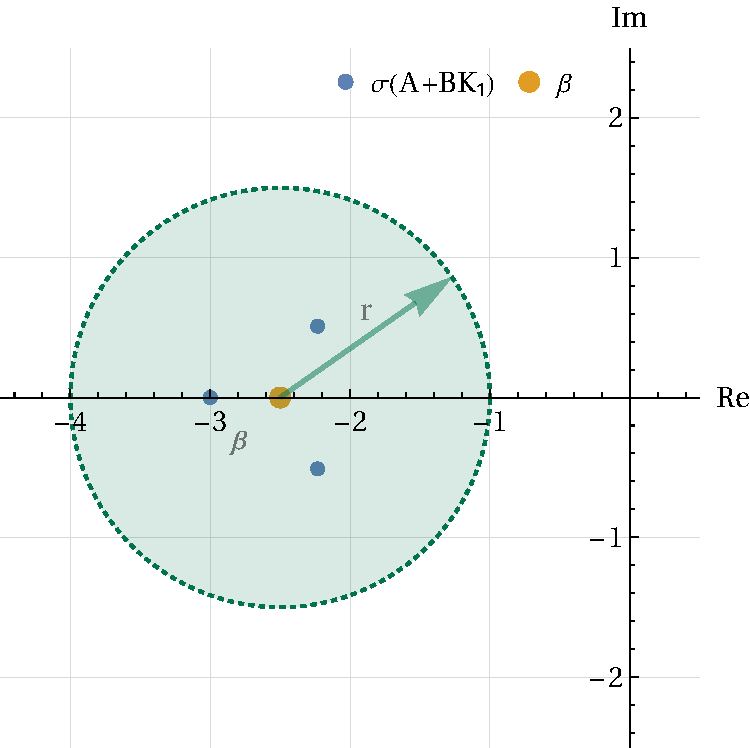
\includegraphics[width=0.5\textwidth]{../images/task3/eig1.pdf}
		\caption{Расположение собственных чисел замкнутой системы}
	\end{figure}
	
	Далее выполню моделирование замкнутой системы при начальных условиях \(x(0) = [1, 1, 1]^\top\). 
	
	\begin{figure}[H]
		\centering
		
\includegraphics[width=0.7\textwidth]{../images/task3/U1.pdf}
		\caption{Управление \(u(t)\)}
	\end{figure}
	
	\begin{figure}[H]
		\centering
		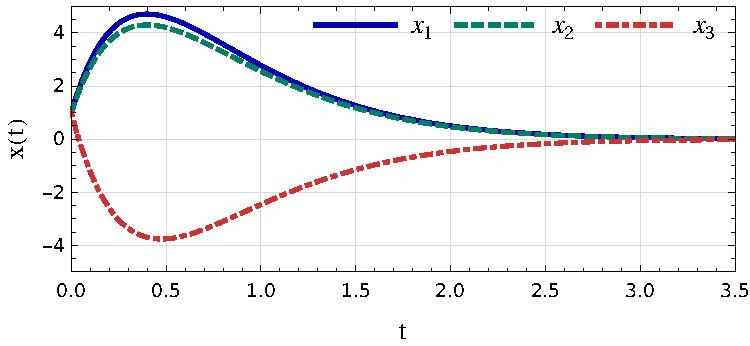
\includegraphics[width=0.7\textwidth]{../images/task3/X1.pdf}
		\caption{Вектор состояния \(x(t)\)}
	\end{figure}
	
По графикам видно, что переходные процессы затухают. Все собственные числа находятся внутри круга, что подтверждает выполнение условия качественной экспоненциальной устойчивости.
	
	\subsection{Набор 2. \(Q = I ,\; R = 0\)}
	
	Синтезирую регулятор \(K_2\) (листинг~\ref{lst:K3}, аналогично):	
	\[
	K_2 = \begin{bmatrix} -2.82 & 0.98 & -2.82 \end{bmatrix}
	\]
	Спектр замкнутой системы:
	\[
	\sigma(A + BK_2) = \{-2.09,\; -2.50 \; -3\}
	\]
	
	Собственные числа на координатной плоскости не выходят на границу круга:
	
	\begin{figure}[H]
		\centering
		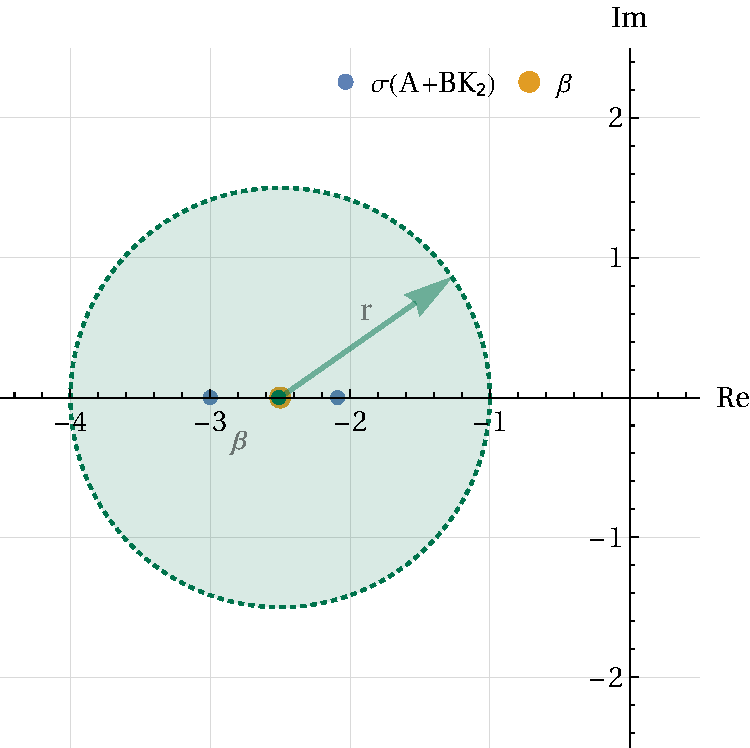
\includegraphics[width=0.5\textwidth]{../images/task3/eig2.pdf}
		\caption{Расположение собственных чисел замкнутой системы}
	\end{figure}
	
	Далее выполню моделирование замкнутой системы при начальных условиях \(x(0) = [1, 1, 1]^\top\). 
	
	\begin{figure}[H]
		\centering
		
\includegraphics[width=0.7\textwidth]{../images/task3/U2.pdf}
		\caption{Управление \(u(t)\)}
	\end{figure}
	
	\begin{figure}[H]
		\centering
		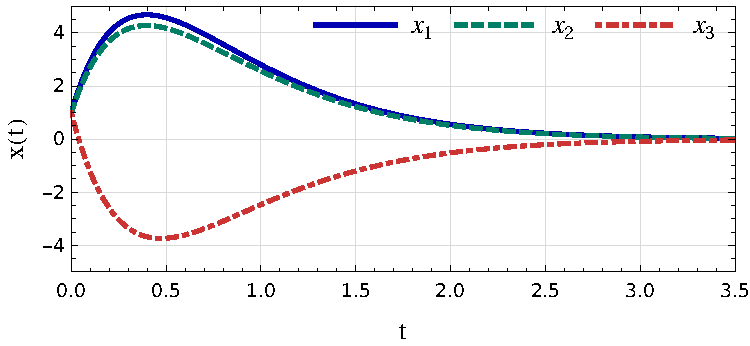
\includegraphics[width=0.7\textwidth]{../images/task3/X2.pdf}
		\caption{Вектор состояния \(x(t)\)}
	\end{figure}
	
	
По графикам видно, что переходные процессы затухают. Все собственные числа находятся внутри круга, что подтверждает выполнение условия качественной экспоненциальной устойчивости.
	
	\subsection{Набор 3. \(Q = 0 ,\; R = 1\)}
	
	Синтезирую регулятор, решая уравнение Риккати (листинг~\ref{lst:K3}, аналогично):	
	\[
	K_3 = \begin{bmatrix} -1.73 & 0.86 & -1.73 \end{bmatrix}
	\]
	
	Спектр замкнутой системы:
	\[
	\sigma(A + BK_3) = \{- 1.02 \pm 0.25\,\mathrm{j},\; -3\}
	\]
	
	Все собственные числа находятся внутри круга с центром \((-2.5, 0)\) и радиусом \(r = 1.5\). Покажу это графически:
	
	\begin{figure}[H]
		\centering
		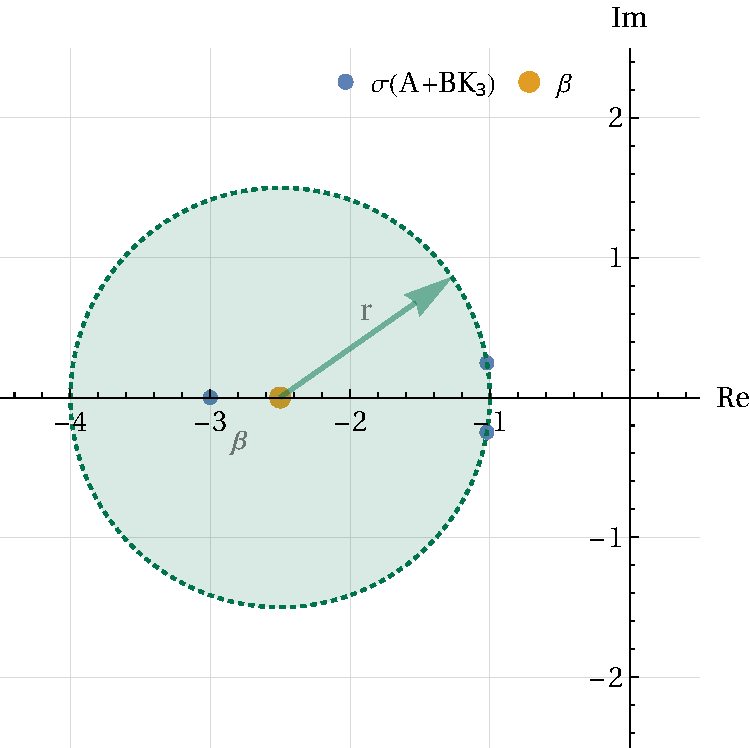
\includegraphics[width=0.5\textwidth]{../images/task3/eig3.pdf}
		\caption{Расположение собственных чисел замкнутой системы}
	\end{figure}
	
	Далее выполню моделирование замкнутой системы при начальных условиях \(x(0) = [1, 1, 1]^\top\). 
	
	\begin{figure}[H]
		\centering
		
\includegraphics[width=0.7\textwidth]{../images/task3/U3.pdf}
		\caption{Управление \(u(t)\)}
	\end{figure}
	
	\begin{figure}[H]
		\centering
		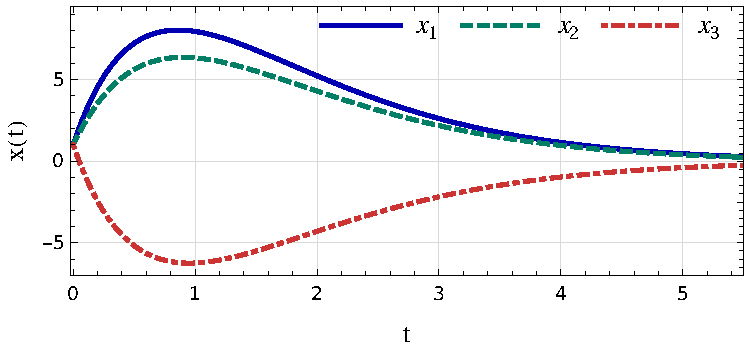
\includegraphics[width=0.7\textwidth]{../images/task3/X3.pdf}
		\caption{Вектор состояния \(x(t)\)}
	\end{figure}
	
		
По графикам видно, что переходные процессы затухают. Все собственные числа находятся внутри круга, что подтверждает выполнение условия качественной экспоненциальной устойчивости.
	
	
	\subsection{Набор 4. \(Q = 0 ,\; R = 0\)}
	
	Синтезирую регулятор, решая уравнение Риккати. Для учёта параметра \(\beta\) делаю замену \(\tilde{A} = A - \beta I\). Получаю:	
	\[
	K_4 = \begin{bmatrix} -2.99 & 0.99 & -2.98 \end{bmatrix}
	\]
	
	Спектр замкнутой системы:
	\[
	\sigma(A + BK_4) = \{-3,\; -2.44,\; -2.5\}
	\]
	
	Собственное число \(\lambda_3 = -3\) находится внутри круга, остальные попали на его границу:
	
	\begin{figure}[H]
		\centering
		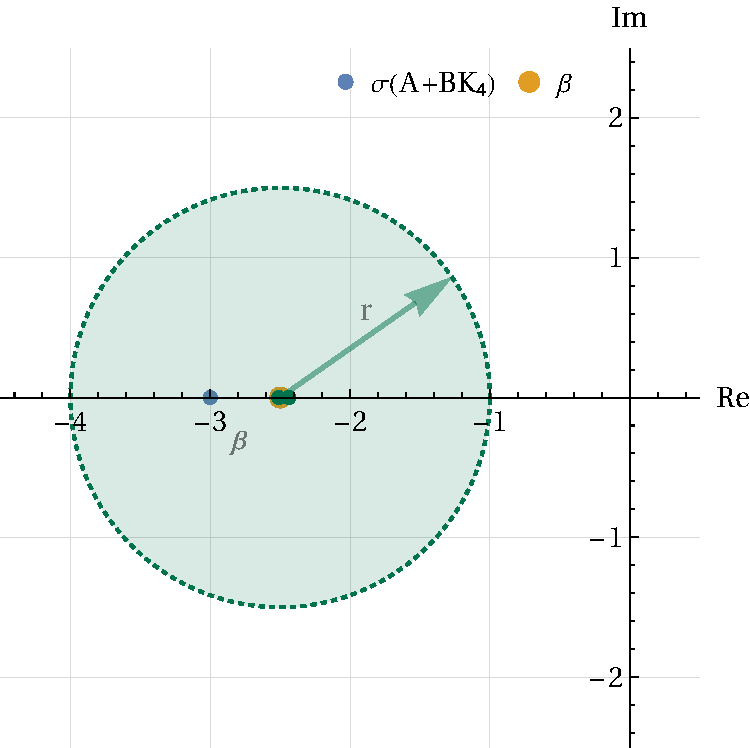
\includegraphics[width=0.5\textwidth]{../images/task3/eig4.pdf}
		\caption{Расположение собственных чисел замкнутой системы}
	\end{figure}
	
	Далее выполняю моделирование замкнутой системы при начальных условиях \(x(0) = [1, 1, 1]^\top\). 
	
	\begin{figure}[H]
		\centering
		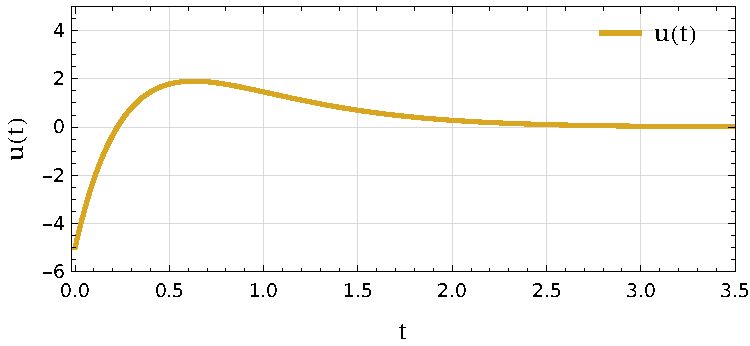
\includegraphics[width=0.7\textwidth]{../images/task3/U4.pdf}
		\caption{Управление \(u(t)\)}
	\end{figure}
	
	\begin{figure}[H]
		\centering
		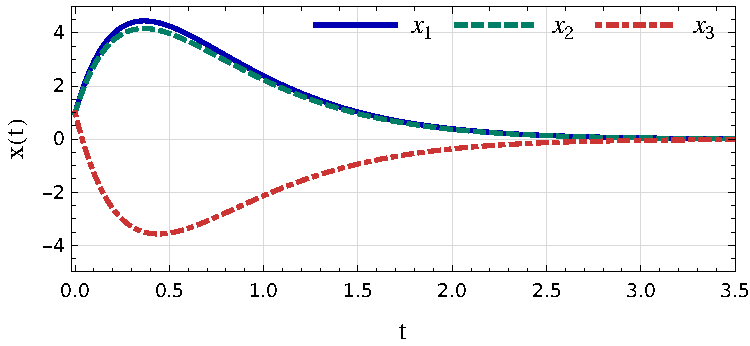
\includegraphics[width=0.7\textwidth]{../images/task3/X4.pdf}
		\caption{Вектор состояния \(x(t)\)}
	\end{figure}
	
	По графикам видно, что переходные процессы затухают. Все собственные числа находятся внутри круга, что подтверждает выполнение условия качественной экспоненциальной устойчивости.
	
	\subsection{Вывод по заданию}
	
	В задании я синтезировала регуляторы для четырёх наборов весовых матриц $Q$ и $R$ при $\beta = -2.5$, $r = 1.5$. Во всех случаях собственные числа замкнутой системы лежат внутри заданного круга, то есть качественная экспоненциальная устойчивость обеспечена. Во всех наборах полученные матрицы регуляторов симметричны (первый и третий коэффициенты равны). Самое медленное затухание наблюдается в наборе 3 ($Q = 0$, $R = 1$). Остальные три набора дают примерно одинаковые и более быстрые переходные процессы.
	
	
	\newpage \section{Вывод}
	
	В ходе работы я синтезировала регуляторы с заданной степенью устойчивости с помощью матричных неравенств Ляпунова и уравнений Риккати, а также построила управление по выходу с наблюдателем полной размерности. Я показала, что изменение весовых матриц $Q$, $R$ и соотношения $\alpha_K$ и $\alpha_L$ меняет интенсивность управления и скорость затухания переходных процессов.
	
	
	
	
	
	
	
	
	
	
	
\newpage
\section{Приложение}

\subsection*{Задание 1}

\begin{lstlisting}[caption={Инициализация}]
A =   
	{{8, 1, 11},
	{4, 0, 4}, 
	{-4, -3, -7}};

B = 
	{{-1}, {-3}, {3}};
\end{lstlisting}

\begin{lstlisting}[caption={Матрица управляемости системы и ее ранг}, label={lst:U1}]
sys = StateSpaceModel[{A, B}];
U = ControllabilityMatrix[sys];
MatrixRank[U]
\end{lstlisting}

\begin{lstlisting}[caption={Жорданова форма системы}, label={lst:jordan1}]
{vals, vecs} = Eigensystem[A]; v = vecs[[2]];
P = Transpose[{vecs[[1]], Re[v], Im[v]}];

Jr = Simplify[Inverse[P].A.P]
Bj = Inverse[P].B
\end{lstlisting}

\begin{lstlisting}[caption={Решение LMI без задачи минимизации}, label={lst:cvx1}, language=Matlab]
A2 = [2 2; -2 2];
B2 = [1.5; -3.5];
a = 0.5;

cvx_begin sdp
	variable P(2,2) symmetric
	variable Y(1,2)
	P >= 0.0001*eye(2);
	P*A2' + A2*P + 2*a*P + Y'*B2' + B2*Y <= 0;
cvx_end

K = Y * inv(P)
Acl = A2 + B2*K;
eig(Acl)
\end{lstlisting}

\begin{lstlisting}[caption={Решение LMI с решением задачи минимизации}, label={lst:cvxmin1}, language=Matlab]
A2 = [2 2; -2 2];
B2 = [1.5; -3.5];
a = 0.5;

cvx_begin sdp
variable P(2,2) symmetric
variable Y(1,2)

minimize(norm(Y))

P >= 0.0001*eye(2);
P*A2' + A2*P + 2*a*P + Y'*B2' + B2*Y <= 0;
cvx_end

K = Y * inv(P)

Acl = A2 + B2*K;
eig(Acl)
\end{lstlisting}

\begin{lstlisting}[caption={Матрица \(K\) в исходном базисе}, label={lst:K1}]
hatK1 = {{0, 1.69, 2.63}};
K1 = hatK1.Inverse[Pj]
\end{lstlisting}

\begin{lstlisting}[caption={Собственные числа замкнутой системы}, label={lst:lEig1}]
Acl = A + B.K1;
Eigenvalues[Acl]
\end{lstlisting}

\begin{lstlisting}[caption={Решение матричного уравнения Риккати при \(Q = I\)}, label={lst:riccati1}]
QI = IdentityMatrix[3];
tildeAa1Q1R = A + alpha1 IdentityMatrix[3];
Pa1Q1R = RiccatiSolve[{tildeAa1Q1R, B}, {QI, R/nu}];
Ka1Q1R = -Inverse[R].Transpose[B].Pa1Q1R

Acla1Q1R = A + B.Ka1Q1R;
Eigenvalues[Acla1Q1R]
\end{lstlisting}

\begin{lstlisting}[caption={Решение матричного уравнения Риккати при \(Q = 0_{3\times3}\)}, label={lst:riccati0}]
Q0 = {{0, 0, 0}, {0, 0, 0}, {0, 0, 0}};
tildeAa1Q0R = A + alpha1 IdentityMatrix[3];
Pa1Q0R = RiccatiSolve[{tildeAa1Q0R, B}, {Q0, R/nu}];
Ka1Q0R = -Inverse[R].Transpose[B].Pa1Q0R

Acla1Q0R = A + B.Ka1Q0R;
Eigenvalues[Acla1Q0R]
\end{lstlisting}
	
	
\newpage \subsection*{Задание 2}

\begin{lstlisting}[caption={Инициализация}]
A = {
	{5, -9, -7, 1}, 
	{-9, 5, -1, 7},
	{-7, -1, 5, 9},
	{1, 7, 9, 5}
};

B = {{3}, {3}, {1}, {3}};

c = {
	{2, -2, 2, 2}, 
	{-2, 4, 2, 4}
};
\end{lstlisting}

\begin{lstlisting}[caption={Переход в жорданов базис}, label={lst:jordan2}]
{P, Aj} = JordanDecomposition[A];
{Bj, Cj} = {Inverse[P].B, c.P};
\end{lstlisting}
	
\begin{lstlisting}[caption={Синтез регулятора \(K\)}, label={lst:K21}]
tildeAaK1 = A + a1K QI;
PaK1 = Round[RiccatiSolve[{tildeAaK1, B}, {QI, R/nu}], 0.01] // N
K1 = Round[-Inverse[R].Transpose[B].PaK1 , 0.01] // N
AclaK1 = A + B.K1; Eigenvalues[Round[AclaK1, 0.01]] // N
\end{lstlisting}

\begin{lstlisting}[caption={Синтез наблюдателя \(L\)}, label={lst:L21}, language=Matlab]
Aj3 = [4 0 0; 0 8 0; 0 0 20];
Cj3 = [0 8 0; 4 0 12];
aL1 = 10;

cvx_begin sdp
	variable Q(3,3) symmetric
	variable Y(3,2)
	
	Q >= 1e-4*eye(3);
	Aj3*Q + Q*Aj3' + 2*aL1*Q + Y*Cj3 + Cj3'*Y' <= 0;
cvx_end

Lj = inv(Q) * Y
\end{lstlisting}

\begin{lstlisting}[caption={Переход в исходный базис}, label={lst:L22}]
Lj1 = {{0, 0}, {0., 7.753}, {-2.2997, 0.}, {0., -6.3768}};
L1 = Round[N[P.Lj1], 0.01];

AclaK1 = A + L1.c;
Eigenvalues[N[AclaK1]]
\end{lstlisting}

\newpage \subsection*{Задание 3}

\begin{lstlisting}[caption={Инициализация}]
A =   
	{{8, 1, 11},
	{4, 0, 4}, 
	{-4, -3, -7}};

B = {{-1}, {-3}, {3}};
x0 = {1, 1, 1};

beta = -2.5;
r = 1.5;
nu = 1;

A1 = A - beta*IdentityMatrix[3];

Q = IdentityMatrix[3];
R = {{1}};
\end{lstlisting}


\begin{lstlisting}[caption={Синтез регулятора \(K\)}. Матрица перехода была найдена в листинге~\ref{lst:jordan1}, label={lst:K3}, language=Matlab]
clear; clc;

A = [8, 1, 11; 4, 0, 4; -4, -3, -7];
B = [-1; -3; 3];

P = [-1, -3, -1; 0, -2, 0; 1, 2, 0];
Aj1 = [2, 2; -2, 2];
Bj1 = [3/2; -7/2];

% Q = eye(2); R = 0;
Q = [0, 0; 0, 0]; R = 0;
b = -2.5; r = 1.5;

syms P_ [2 2]
K_ = -(inv(R + Bj1' * P_ * Bj1) * Bj1' * P_ * (Aj1 - b*eye(2)));
eqs = (Aj1 + Bj1*K_ - b*eye(2))' * P_ * (Aj1 + Bj1*K_ - b*eye(2)) - r^2 * P_ == -Q;
s = vpasolve(eqs, [P_], Random=true);
P_ = [s.P_1_1, s.P_1_2; s.P_2_1, s.P_2_2];

K = round([0, -(inv(R + Bj1' * P_ * Bj1) * Bj1' * P_ * (Aj1 - b*eye(2)))] * P^-1, 4);
e = round(eig(A + B*K), 4);
dists = abs(e - b);

if all(real(e) < 0) && all(dists < r)
	disp('K ='); disp(K);
	disp('e ='); disp(e);
else
	disp('no');
end
\end{lstlisting}
	
\end{document}